\documentclass[11pt,a4paper]{article}

\usepackage[T1]{fontenc}
\usepackage{lmodern}
\usepackage[margin=1in]{geometry}
\usepackage{amsmath,amssymb,amsthm,mathtools}
\usepackage{microtype}
\usepackage{booktabs}
\usepackage{array}
\usepackage{graphicx}
\usepackage[section]{placeins}
\usepackage{xcolor}
\usepackage{url}
\def\UrlBreaks{\do\/\do\-\do\_\do\.}
\usepackage{enumitem}
\usepackage[colorlinks=true,linkcolor=blue!60!black,citecolor=teal!60!black,urlcolor=blue!60!black]{hyperref}
\usepackage[nameinlink,capitalise]{cleveref}

\numberwithin{equation}{section}

\theoremstyle{plain}
\newtheorem{theorem}{Theorem}[section]
\newtheorem{proposition}[theorem]{Proposition}
\newtheorem{lemma}[theorem]{Lemma}
\newtheorem{corollary}[theorem]{Corollary}

\theoremstyle{definition}
\newtheorem{definition}[theorem]{Definition}

\theoremstyle{remark}
\newtheorem{remark}[theorem]{Remark}

\newcommand{\N}{\mathbb{N}}
\newcommand{\Z}{\mathbb{Z}}
\newcommand{\Q}{\mathbb{Q}}
\newcommand{\R}{\mathbb{R}}
\newcommand{\C}{\mathbb{C}}
\newcommand{\Qp}{\mathbb{Q}_p}
\newcommand{\Zp}{\mathbb{Z}_p}
\newcommand{\Tp}{T_p}
\newcommand{\Dp}{D_p^\alpha}
\newcommand{\IPR}{\mathrm{IPR}}
\newcommand{\lca}{\mathrm{lca}}
\newcommand{\Aut}{\mathrm{Aut}}
\newcommand{\code}[1]{{\ttfamily\footnotesize\def\_{\textunderscore\penalty0\hskip0pt}#1}}
\emergencystretch=4em

\title{\Large\bfseries ULTRAMETRICA: Exact Non-Archimedean Holography, Recursive Adelic Valuation-Residue Symmetries, Multi-Edge Bridge Ollivier--Ricci Metric-Invariance, Graph-Cut Strong Subadditivity, and Lean~4 Checked Model Invariants}

\author{
  Alexander Stephen Donahue\thanks{Independent Researcher (project handle \texttt{0thernes}), Spokane, WA, USA. Email: \href{mailto:0_0@0thernes.art}{\texttt{0\_0@0thernes.art}}. ORCID: \href{https://orcid.org/0009-0006-8168-9648}{\texttt{0009-0006-8168-9648}}. Source code, formal proofs, claim ledger, and preregistration: \url{https://github.com/0thernes/ultrametrica}. Live WebGL2 observatory: \url{https://0thernes.github.io/ultrametrica/}.}\\[0.35em]
  \normalsize Independent Researcher, Spokane, WA, USA
}

\date{November 27, 2026 (Version 1.8.1)}

\begin{document}

\maketitle

\begin{abstract}
We present \textbf{ULTRAMETRICA} (\code{v1.8.1}), a zero-dependency computational laboratory and formal mathematical framework for a discrete $p$-adic AdS/CFT (Bruhat--Tits tree) holography model coupling discrete $p$-adic boundary dynamics on $\Zp / p^n \Zp$ ($p \in \{2,3,5,7\}$) to exact discrete bulk scalar fields on the Bruhat--Tits tree $\Tp$ and its rotating Tate-curve BTZ black hole quotients $\Tp / p^{h\Z}$. Beyond implementing established non-Archimedean constructions to machine precision ($10^{-12}$--$10^{-17}$, tagged \code{numerical\_\allowbreak approximation} in IEEE-754 float64)---including native Radix-$p$ Pontryagin fast Fourier transforms, Vladimirov fractional pseudo-differential operators $\Dp$, orthonormal Kozyrev wavelets, fourth-order Yoshida symplectic nonlinear integration, Johnson potential-reduced Dijkstra $1$-Wasserstein transport on curved BTZ horizons, symmetric Jacobi dynamic edge-length backreaction, and exact $O(V)$ Ryu--Takayanagi minimal cuts---we derive, independently cross-check in exact arbitrary-precision rational arithmetic, stress-test against $36$ Node suites ($12/12$ real source-code mutants killed against unmodified \code{test/\allowbreak verify.mjs}, $3{,}400+$ seeded property and curved-BTZ distortion checks, $1{,}000$ deterministic HTTP/engine fuzz cases, and $3$ parallel HTTP/\code{AudioWorklet} concurrency suites), confirm via a git-sealed pre-registered $20$-seed statistical falsification experiment (with Mann--Whitney~$U$, $95\%$ bootstrap CIs for all three effect sizes, and non-pseudoreplicated matrix-level Wilcoxon tests; deviations logged in \code{DEVIATIONS.md}), and machine-verify $250$ audited discrete model declarations in pure Lean~4 (\code{v4.35.0}, Palomar \code{module} headers, zero Mathlib, \code{autoImplicit = false}, zero \code{native\_\allowbreak decide}, no \code{sorry} outside statement-only \code{Challenge.lean}, all $17$ files $< 1{,}000$ lines, $100.0\%$ public theorem axiom audit coverage)---transparently accounted as $144$ core theorems and corollaries, $81$ zero-Mathlib helper lemmas, $10$ kernel-checked adversarial false-variant refutations, and $15$ isolated \code{Spec}/\code{Challenge}/\code{Solution} comparator bindings (never double-counted as extra discoveries; all $250$ checked by Lean and \code{leanchecker {-}{-}fresh}, with all $15$ comparator targets and their dependency closure verified across $6$ independent kernels via \code{lake comparator {-}{-}paranoid} plus a live negative tamper-rejection gate in CI). Building on our \code{v1.7.0} baseline, \code{v1.8.x} closes three remaining discrete formalization boundaries inside pure Lean~4: (a)~full-graph $(p+2)\times(p+2)$ unicyclic BTZ symmetry reduction and primal--dual optimal transport (\code{FullGraphBTZ.lean}, Target~13); (b)~operator-level matrix block-diagonality and odd-prime orthogonal conjugate eigenvector multiplicity $\ge 2$ over $\Z[i]^N$ (\code{OperatorAndSpectrum.lean}, Target~14); and (c)~finite weighted gauge-covariant graph Laplacian strict positive definiteness $T \succ 0$, end-to-end Sherman--Morrison $\mathrm{den} \ge 1$ discharge, and exact rational (\code{RatQ}) tree Schur-complement pivot positivity (\code{BulkOperatorPositivity.lean}, Target~15). Lean still operates over exact algebraic rings ($\Z, \Z[i], \text{\code{RatQ}}$) rather than floating-point/continuum manifolds: it does not formalize the full irrational-root DFT matrix $H_\theta$, continuum PDE time evolution, the floating-point $O(V)$ JS solver, or tachyonic negative-mass BF-window positivity (see \cref{tab:claims}). Across seven formal/computational result families and nine reproducible experiments (Experiments~A--I):
\begin{enumerate}[leftmargin=1.8em,itemsep=2pt]
  \item \emph{Adelic Parity-Doubling, Operator-Level Multiplicity $\ge 2$, and Pre-Registered GOE/GUE Falsification (\cref{thm:adelic}, \cref{prop:picket}, \cref{tab:expi}):} Conjugating $\Dp$ by the universal base-$p$ Monna digit-reversal involution $R_p$ (Monna~\cite{Monna1970}) and adding any real even circulant operator $H_{\R}$ produces a non-commuting hybrid $H_\theta = \theta R_p \Dp R_p + (1-\theta) H_{\R}$ that block-diagonalizes identically into $1 + n(p-1)$ Fourier sectors $W_{s,m}$ (paper proof + numerical off-block leak $\le 1.8\times 10^{-14}$ up to $N = 625$; Lean verifies Monna involution, ball contiguity, subtree-shift prefixes, $[D_K, J] = 0$ parity preservation, diagonal-commuting matrix block-diagonality, odd-prime strictly orthogonal linearly independent Fourier-conjugate eigenvector doublets over $\Z[i]^N$ with multiplicity $\ge 2$, and the closed-form picket-fence sequence), enforcing even multiplicity for odd primes $p \ge 3$ while lifting all doublets to $2^n$ simple levels at $p = 2$. Pre-registered Experiment~I rejects Wigner--Dyson GOE/GUE thermalization across all $4/4$ hypotheses ($20/20$ seeds each, Holm--Bonferroni $p_{\mathrm{Holm}} = 0.0004$).
  \item \emph{Full-Graph Tate-Curve BTZ Ollivier--Ricci Law and $L_c = 5$ Trichotomy (\cref{thm:btz-ricci}):} For all $p \ge 2, L \ge 3$, every horizon edge obeys $\kappa_{\mathrm{BTZ}}(p, L) = -(2p - \max(0, 6-L))/(p+2)$, establishing Planck-scale flattening ($L \in \{3,4\}$, and $L=5$ for $p \ge 4$), exact zero excess at $(p, L) = (3, 5)$, and macroscopic deficit $-4/((p+1)(p+2))$ for $L \ge 6$ (Lean~4 now certifies BOTH the $3$-class reduced model AND the literal $(p+2)\times(p+2)$ full-graph symmetry reduction, universal lower bound, and explicit non-negative full-graph optimal transport plan in \code{FullGraphBTZ.lean}, Target~13, cross-checked over $45$ exact \code{Fraction} full-graph solves).
  \item \emph{Single-Edge, Multi-Edge, and Finite-Graph Bridge Ollivier--Ricci Metric-Invariance and Pinch Deficit (\cref{thm:gauss-bonnet}, \cref{thm:gauss-bonnet-global}, \cref{rem:gubser-non-topological}):} For \emph{arbitrary simultaneous finite-support positive conductances} $w_e = 1/a_e > 0$ on strictly interior bridge edges of $\Tp$ (prime integer $p \ge 2$, $(p+1)$-regular), non-lazy ($t = 1$) conductance Ollivier--Ricci curvature obeys an exact two-branch law with subcritical metric-invariance ($\Delta\sum_e \kappa_e \equiv 0$ whenever $w_e/W_u + w_e/W_v \le 1$, via local vertex probability-normalization telescoping) and a strictly negative supercritical pinch deficit $-2\sum_e \max(0, w_e/W_u + w_e/W_v - 1)$ beyond threshold. Lean~4 certifies both the arbitrary-degree inhomogeneous bridge Kantorovich primal--dual bounds with kernel-verified non-negative plans and direct edge-sum double-counting over arbitrary finite undirected weighted edge lists on $\mathrm{Fin}\,n$ (\code{FiniteGraph\allowbreak GaussBonnet.\allowbreak lean}, Target~11), yielding $\sum_{e\in E}\kappa_e = -(p-1)n - \sum_{e\in E}\mathrm{def}_e$ in exact rational arithmetic (contrasted explicitly with Gubser et~al.'s~\cite{GubserEdge2017} $t\to 0^+$ lazy $J_e = a_e^{-2}$ action and distinguished from topological Gauss--Bonnet in \cref{rem:gubser-non-topological}; cross-checked over $69$ exact \code{Fraction} plans and $1{,}000$ random multi-edge trees to $< 10^{-11}$).
  \item \emph{Discrete Vladimirov / Kozyrev--Haar Eigenfunctions, Multi-Ball Compacton-Solitons, and Self-Trapping (\cref{thm:vladimirov-kozyrev}, \cref{thm:soliton}):} For every $p \ge 2$, depth $n$, scale $j < n$, ball center $c < p^n$, zero-sum profile $a : \mathrm{Fin}\,p \to \Z$, and arbitrary radial ultrametric kernel $K : \N \to \Z$ (covering cleared-denominator $\Dp$), Lean~4 proves from first principles that the discrete Kozyrev--Haar wavelet $\psi_{j,c,a}$ is an exact eigenfunction of $D_K$ with scale-only eigenvalue and that $[D_K, J] = 0$ preserves even/odd parity (\code{VladimirovOperator.lean}, Target~12; extending to complex character profiles by $\C$-linearity). Combined with kernel-checked $K$-ball pointwise nonlinearity splitting over $\Z[i]$, disjoint Kozyrev superpositions evolve without cross-ball leakage under $i\partial_t \psi = (\Dp + F(|\psi|^2))\psi$ (PDE dynamics verified numerically with $0.00\%$ leakage up to $g = 500$), whereas overlapping multi-scale packets show monotonic $\alpha$-decaying resonant peaks and universal large-$g$ self-trapping.
  \item \emph{Bulk Operator Positivity ($T \succ 0$), Tree Schur Pivots, Rank-$1$ Kerr--BTZ Solver, Flux Parity, and BF Margin (\cref{thm:solver}):} Decomposing the rotating horizon wrap edge as $w_{L-1} u u^\dagger \succeq 0$ yields an $O(V)$ complex Hermitian Sherman--Morrison solver with $\mathrm{den} \ge 1$ whenever $T \succ 0$. Lean~4 now proves strict positive definiteness of every finite weighted gauge-covariant graph Laplacian with strictly positive diagonal ($m^2 > 0$ or positive Robin shift), discharges $\mathrm{den} \ge 1$ and $\mathrm{den} \ne 0$ directly from $T \succeq 0$, proves exact \code{RatQ} tree Schur-complement pivot positivity $D_p - w^2/D_c > 0$ and exact elimination (\code{BulkOperatorPositivity.lean}, Target~15), and certifies the arbitrary-dimension Sherman--Morrison identity and edge-level flux parity; the floating-point $O(V)$ solver and tachyonic BF-window stability down to $\Delta = 0.5001, \Omega = \pi$ (residual $\le 5.38\times 10^{-15}$) are verified in exact $\Q(i)$ and float64.
  \item \emph{Discrete Graph-Cut Strong Subadditivity (\cref{thm:rt-ssa}):} Formalized in Lean~4 for \emph{arbitrary} finite \code{Nat}-weighted graphs under cut-minimality hypotheses, minimal homologous cuts obey $S(A \cup B \cup C) + S(B) \le S(A \cup B) + S(B \cup C)$ for all disjoint boundary regions $A, C$ (discrete formalization of Headrick--Takayanagi~\cite{HeadrickTakayanagi2007}, no priority claimed; independently confirmed over $4{,}352$ exhaustive brute-force partitions and $1{,}000$ random JS graphs).
\end{enumerate}
\end{abstract}

\medskip
\noindent\textbf{Keywords:} $p$-adic AdS/CFT; Bruhat--Tits tree; Vladimirov operator; Kozyrev wavelets; adelic physics; Ollivier--Ricci curvature; Kantorovich duality; BTZ black hole; Ryu--Takayanagi strong subadditivity; Lean~4 verification.

\smallskip
\noindent\textbf{MSC 2020:} 11S80; 81T40; 83E05; 05C12; 42C40; 68V20.

\tableofcontents

% =====================================================================
\section{Introduction, Epistemic Scope, and Claims Summary}
\label{sec:intro}
% =====================================================================

By Ostrowski's theorem, every non-trivial absolute value on $\Q$ is equivalent either to the Archimedean norm $|\cdot|_\infty$ (completing to $\R$) or to a $p$-adic ultrametric norm $|x|_p = p^{-v_p(x)}$ for some prime $p$ (completing to $\Qp$), obeying the strong triangle inequality $|x + y|_p \le \max(|x|_p, |y|_p)$. Non-Archimedean and adelic models of Planck-scale geometry and string amplitudes were pioneered by Volovich~\cite{Volovich1987}, Freund and Witten~\cite{FreundWitten1987}, and Vladimirov, Volovich, and Zelenov~\cite{Vladimirov1994}, with comprehensive modern surveys in~\cite{Dragovich2017}. A structural resurgence followed the formulation of \emph{$p$-adic AdS/CFT} by Gubser et~al.~\cite{Gubser2017,GubserEdge2017} and Heydeman, Marcolli, Saberi, and Stoica~\cite{Heydeman2018,Heydeman2021}, establishing the $(p+1)$-regular Bruhat--Tits tree $\Tp$ as a discrete hyperbolic holographic bulk dual to $\mathbb{P}^1(\Qp)$ and its Tate-curve Schottky quotients $\Tp / q^{\Z}$ as discrete BTZ black holes.

\textbf{Epistemic and Priority Scope.} This manuscript is an independent mathematical-physics, formal-verification, and computational engineering preprint; it is \emph{not} a peer-reviewed journal article and makes no claim of empirical discovery of new physical laws of nature. Foundational $p$-adic analysis, Kozyrev wavelets~\cite{Kozyrev2002}, $p$-adic AdS/CFT~\cite{Gubser2017,Heydeman2018}, dynamic edge-length gravity~\cite{GubserEdge2017}, Ollivier--Ricci curvature on regular trees~\cite{Ollivier2009,LinLuYau2011}, holographic entanglement entropy and strong subadditivity~\cite{RyuTakayanagi2006,HeadrickTakayanagi2007,Pastawski2015}, random-matrix spacing ratios~\cite{OganesyanHuse2007,Atas2013}, Holm--Bonferroni correction~\cite{Holm1979}, fourth-order Yoshida splitting~\cite{Yoshida1990}, and the Lean~4 theorem prover~\cite{deMouraUllrich2021} are credited to their original authors. Furthermore, a systematic cross-check against all $1{,}900$ open problems in \code{0thernes/unsolved-problems-mega-atlas} (archived in \code{docs/\allowbreak MEGA\_ATLAS\_CROSSCHECK.md}) establishes honestly that ULTRAMETRICA solves \emph{zero} ($0/1{,}900$) open problems completely; it supplies exact discrete finite-cutoff sub-results related to \code{SUB-032} ($p$-adic AdS/CFT) and a pre-registered negative result falsifying naive GOE/GUE thermalization in Monna-conjugated adelic hybrids. \Cref{tab:claims} summarizes every original claim together with its exact verification tier.

\begin{table}[ht]
\centering
\caption{Numbered Claims Summary Table separating verification tiers explicitly (mapped 1-to-1 with falsification criteria in root \code{CLAIMS.md}; floating-point evaluations tagged \code{numerical\_approximation}).}
\label{tab:claims}
\footnotesize
\setlength{\tabcolsep}{3.2pt}
\begin{tabular}{@{}l>{\raggedright\arraybackslash}p{5.0cm}>{\raggedright\arraybackslash}p{3.1cm}>{\raggedright\arraybackslash}p{4.3cm}@{}}
\toprule
ID & Statement Summary & Verification Tier & Primary Artifact \\
\midrule
C1 & Monna involution $R_p$, ball contiguity, subtree-shift prefixes, $[D_K,J]=0$ parity, matrix block-diagonality, and odd-prime orthogonal doublet multiplicity $\ge 2$ (\cref{thm:adelic}) & kernel (Monna, shifts, $J$-parity, block-diag, $\Z[i]^N$ doublets); exact-rat./num.\ (DFT $H_\theta$) & \code{Basic.lean}, \code{Adelic\allowbreak Symmetry.lean}, \code{OperatorAnd\allowbreak Spectrum.lean}, \code{Vladimirov\allowbreak Operator.lean} \\
C2 & Alternating picket-fence gaps $p-2m, 2m$ and $\alpha$-invariant ratio $r_0(p,m)$ (\cref{prop:picket}) & kernel (sequence); exact-rat./num.\ (eigenvalues, $\alpha$) & \code{AdelicSymmetry.lean}, Exp~E \& G \\
C3 & Pre-registered 20-seed rejection of GOE/GUE thermalization across H1--H4 ($p_{\mathrm{Holm}} = 0.0004$, matrix Wilcoxon $p_{\mathrm{Holm}} = 7.63\times 10^{-6}$) & pre-registered statistical & \code{docs/preregistration.md} (\code{c171b1b}), \code{DEVIATIONS.md}, \code{stats-eval.json} \\
C4 & Tate-curve $L$-cycle BTZ Ollivier--Ricci law, full $(p+2)\times(p+2)$ symmetry reduction, and $L_c = 5$ trichotomy (\cref{thm:btz-ricci}) & kernel (3-class + full-graph $(p+2)\times(p+2)$); exact-rat./num. & \code{Holography\allowbreak Curvature.lean}, \code{FullGraphBTZ.lean}, 45 \code{Fraction} plans, Mutant M3 \\
C5 & Single-edge, multi-edge, and finite-graph bridge Ollivier--Ricci subcritical metric-invariance \& pinch deficit (\cref{thm:gauss-bonnet,thm:gauss-bonnet-global,rem:gubser-non-topological}) & kernel (per-edge, per-vertex \& finite-graph edge sum); exact-rat./num. & \code{MultiEdge\allowbreak Holography.lean}, \code{FiniteGraph\allowbreak GaussBonnet.lean}, 69 \code{Fraction} plans \\
C6 & Discrete Vladimirov / Kozyrev--Haar eigenfunctions (\cref{thm:vladimirov-kozyrev}) \& $K$-ball compacton-soliton invariance (\cref{thm:soliton}) & kernel ($D_K$, Kozyrev--Haar, $\Z[i]$ split); numerical\_\allowbreak approx.\ (PDE) & \code{Vladimirov\allowbreak Operator.lean}, \code{SolitonAnd\allowbreak Solver.lean}, Exp~C \& F \\
C7 & Bulk Laplacian $T \succ 0$, \code{RatQ} tree Schur pivots, Rank-1 Kerr--BTZ solver ($\mathrm{den} \ge 1$), flux parity, and BF stability ($\Delta = 0.5001$) (\cref{thm:solver}) & kernel ($T \succ 0$, Schur pivots, $\mathrm{den}\ge 1$, alg.\ core); exact-rat./num.\ (JS solver, BF) & \code{SolitonAnd\allowbreak Solver.lean}, \code{BulkOperator\allowbreak Positivity.lean}, exact $\Q(i)$ solve, Exp~D \& H \\
C8 & Discrete weighted-graph holographic RT Strong Subadditivity (\cref{thm:rt-ssa}; Headrick--Takayanagi~\cite{HeadrickTakayanagi2007}) & kernel-checked, exact-rational, numerical\_\allowbreak approx. & \code{MultiEdgeHolography.lean}, 4,352 brute-force + 1,000 props \\
C9 & Real-time zero-dependency engine (Dijkstra BTZ $W_1$, $12/12$ real source mutants, 100\% Lean public theorem coverage, dual timestamps) & numerical\_\allowbreak approx. (contract, fuzz, race) & \code{test/*.mjs} (36/36), \code{padic\_oracle.py}, \code{stamp\_manifest.py} \\
\bottomrule
\end{tabular}
\end{table}

% =====================================================================
\section{Discrete \texorpdfstring{$p$}{p}-adic Harmonic Analysis and Universal Monna Geometry}
\label{sec:padic}
% =====================================================================

Fix a prime $p \in \{2,3,5,7\}$ and precision depth $n \ge 2$, with dimension $N = p^n$. We discretize locally constant Schwartz--Bruhat functions on $\Zp$ to the finite-dimensional Hilbert space $\mathcal{H}_{p,n} = L^2(\Zp / p^n \Zp) \cong \C^{p^n}$.

\subsection{Universal Base-\texorpdfstring{$p$}{p} Digit Reversal and Ball Contiguity}
Write $x \in \{0,\dots,p^n - 1\}$ in little-endian base-$p$ digits $x = \sum_{r=0}^{n-1} d_r p^r$ ($d_r \in \{0,\dots,p-1\}$). The classical Monna map~\cite{Monna1970} $\mathcal{M}_p : \Zp \to [0,1]$ sends $x \mapsto \sum_{r=0}^{n-1} d_r p^{-(r+1)}$. On $\Z / p^n\Z$, scaling by $p^n$ yields the exact \emph{base-$p$ digit-reversal involution}
\begin{equation}
  R_p(x) := p^n \mathcal{M}_p(x) = \sum_{r=0}^{n-1} d_r p^{n-1-r}, \qquad R_p(R_p(x)) = x.
  \label{eq:monna-inv}
\end{equation}
In \code{UltrametricaProofs/Basic.lean}, we prove \emph{universally} for all integers $p \ge 2$, all depths $n \in \N$, and all $x, y < p^n$ (replacing finite enumeration with structural induction):
\begin{enumerate}[leftmargin=1.8em,itemsep=1pt]
  \item $R_p(R_p(x)) = x$, together with explicit injectivity and surjectivity on $\{0,\dots,p^n-1\}$ (\code{monna\_involution\_universal}, \code{monna\_injective}, \code{monna\_surjective});
  \item $R_p(p^n - 1 - x) = p^n - 1 - R_p(x)$ (\code{complement\_commutes\_monna\_universal});
  \item $x \equiv y \pmod{p^j} \iff \lfloor R_p(x) / p^{n-j} \rfloor = \lfloor R_p(y) / p^{n-j} \rfloor$ and $p^j p^{n-j} = p^n$ for all $j \le n$ (\code{padic\_ball\_monna\_contiguity}, \code{padic\_ball\_cardinality});
  \item a concrete kernel-checked \code{Ultrametric Nat} instance \code{bruhatTitsUltrametric} for the tree-hop geodesic distance \code{treeHopDist} on $\Tp$, instantiating the universal isosceles triangle theorem directly on Bruhat--Tits leaves (\code{bruhatTits\_leaves\_isosceles}).
\end{enumerate}

\subsection{Native Radix-\texorpdfstring{$p$}{p} Pontryagin FFT and Vladimirov Operator}
The Pontryagin dual of $\Zp / p^n\Zp$ is $p^{-n}\Z / \Z$, indexed by $k \in \{0,\dots,p^n-1\}$ with additive character $\chi_p(\xi_k x) = e^{2\pi i k x / p^n}$ ($\xi_k = k/p^n$). To preserve exact prime-power periodicity without power-of-$2$ zero-padding artifacts, \code{src/engine/padic.js} implements a native decimation-in-time unitary Radix-$p$ Cooley--Tukey transform:
\begin{equation}
  (\mathcal{F}_p \psi)[k] = \frac{1}{\sqrt{p^n}} \sum_{x=0}^{p^n-1} \psi(x) e^{-2\pi i x k / p^n}
  \label{eq:radix-fft}
\end{equation}
in $O(p N \log_p N)$ operations, verified against naive $O(N^2)$ DFT, an independent textbook Python differential oracle (\code{reference/padic\_oracle.py}, $1{,}000$ Monna/ultrametric queries + $40$ full Vladimirov DFTs, max error $1.23\times 10^{-12}$), and Parseval's identity across $p \in \{2,3,5,7\}$, achieving $7.76\times$ ($N=9$), $159.47\times$ ($N=243$), and $280.2\times$ ($N=625$) median speedups over naive DFT (\code{results/perf-benchmarks.json}). The Vladimirov fractional pseudo-differential operator $\Dp$~\cite{Vladimirov1994} acts diagonally in Pontryagin dual space via
\begin{equation}
  \widehat{(\Dp \psi)}[k] = |\xi_k|_p^\alpha \, \hat{\psi}[k], \qquad
  |\xi_k|_p = \begin{cases} 0 & k = 0, \\ p^{n - v_p(k)} & 1 \le k < p^n, \end{cases}
  \label{eq:vladimirov}
\end{equation}
where $v_p(k) = \max\{r : p^r \mid k\}$. Its position-space matrix elements depend strictly on $v_p(x - y)$ (verified to $1.78\times 10^{-15}$), endowing $\Dp$ with symmetry under the entire Bruhat--Tits wreath-product automorphism group $\Aut(\Tp) = S_p \wr \cdots \wr S_p$.

% =====================================================================
\section{Kozyrev Wavelets and Multi-Ball Compacton-Soliton Invariance}
\label{sec:solitons}
% =====================================================================

Kozyrev~\cite{Kozyrev2002} constructed an orthonormal basis of strictly compactly supported eigenfunctions of $\Dp$. On $\Zp / p^n\Zp$, for scale $0 \le j < n$, ball $0 \le b < p^j$, and non-trivial character $1 \le m < p$:
\begin{equation}
  \psi_{j,b,m}(x) = p^{-(n-j)/2} \, \mathbf{1}_{B_j(b)}(x) \, \exp\!\left(\frac{2\pi i \, m \, d_j(x)}{p}\right),
  \qquad \Dp \psi_{j,b,m} = p^{\alpha(j+1)} \psi_{j,b,m}.
  \label{eq:kozyrev}
\end{equation}
Together with the constant mode $\psi_0(x) = p^{-n/2}$, the total count satisfies $1 + \sum_{j=0}^{n-1}(p-1)p^j = p^n$ (Lean~4: \code{hilbert\_sector\_completeness}). Unlike Euclidean space---where Paley--Wiener analyticity forbids compactly supported eigenfunctions of $(-\Delta_{\R})^{\alpha/2}$---Kozyrev localization holds algebraically for \emph{every} discrete radial ultrametric convolution operator and extends verbatim to arbitrary local nonlinearities.

\begin{theorem}[First-Principles Discrete Vladimirov / Kozyrev--Haar Eigenfunctions and $J$-Parity]
\label{thm:vladimirov-kozyrev}
Fix any integer $p \ge 2$, depth $n \ge 1$, scale $0 \le j < n$, ball center $c < p^n$, radial kernel $K : \N \to \Z$, and zero-sum child profile $a : \mathrm{Fin}\,p \to \Z$ ($\sum_{d=0}^{p-1} a_d = 0$). Define the exact finite-level ultrametric convolution operator $(D_K f)(x) := \sum_{y=0}^{p^n - 1} K(v_p^{(n)}(x - y))\, f(y)$ (instantiating cleared-denominator $\Dp$) and the discrete Kozyrev--Haar wavelet $\psi_{j,c,a}(x) := \mathbf{1}_{x \equiv c \pmod{p^j}}\, a_{\lfloor x/p^j\rfloor \bmod p}$ on $\Z/p^n\Z$. Then:
\begin{enumerate}[leftmargin=1.8em,itemsep=1pt]
  \item $v_p^{(n)}$ satisfies the exact strong ultrametric triangle and sharp isosceles laws on $\Z/p^n\Z$, and $\sum_{x} \psi_{j,c,a}(x) = 0$;
  \item for every $x \in \Z/p^n\Z$, $(D_K \psi_{j,c,a})(x) = \lambda_K(p,n,j)\,\psi_{j,c,a}(x)$ with exact scale-only eigenvalue $\lambda_K(p,n,j) = \sum_{t=0}^{p^{n-j-1}-1} K(j + 1 + v_p^{(n-j-1)}(t)) - p^{n-j-1} K(j)$ (strictly independent of $c$ and $a$; extending by $\C$-linearity to complex Kozyrev characters $a_d = e^{2\pi i m d/p}$ whose real and imaginary parts each sum to zero);
  \item $D_K$ commutes identically with the complement-reversal involution $(J f)(x) = f(p^n - 1 - x)$, and every $J$-commuting negation-preserving operator preserves both even and odd parity subspaces.
\end{enumerate}
\end{theorem}

\begin{proof}
Outside the support ball $B(c, j)$, the sharp ultrametric isosceles law forces $v_p^{(n)}(x - y) = v_p^{(n)}(x - c)$ identically for all $y \in B(c, j)$, factoring $K(v_p^{(n)}(x-c))$ outside the zero-mean sum. Inside $B(c, j)$, reindexing $y = (q p + d)p^j + r$ collapses $r$ to $c \bmod p^j$, yields exact valuation $j$ across all sibling sub-balls $d \ne d_0$, and maps the same-sub-ball sum $d = d_0$ via a modular subtraction bijection to $\sum_t K(j + 1 + v_p(t))$, where subtracting $p^{n-j-1} K(j)\sum_d a_d = 0$ isolates $\lambda_K(p,n,j)\,a_{d_0}$. Complement invariance $v_p^{(n)}((p^n-1-x)-(p^n-1-y)) = v_p^{(n)}(x-y)$ gives $[D_K, J] = 0$. All parts are kernel-checked from first principles in \code{UltrametricaProofs/\allowbreak VladimirovOperator.lean} (\code{padicDistVal\_\allowbreak strong\_\allowbreak tri}, \code{kozyrevHaar\_\allowbreak zero\_\allowbreak mean}, \code{kozyrevHaar\_\allowbreak vladimirov\_\allowbreak eigenfunction}, \code{ultrametricOp\_\allowbreak commutes\_\allowbreak vecRev}, \code{j\_\allowbreak commuting\_\allowbreak preserves\_\allowbreak parity}, and isolated 6-kernel comparator target \code{target\_\allowbreak thm7\_\allowbreak vladimirov\_\allowbreak kozyrev\_\allowbreak eigenfunction}; sharpness of $\sum a = 0$ is proved by \code{adv\_\allowbreak nonzerosum\_\allowbreak not\_\allowbreak vladimirov\_\allowbreak eigenfunction}).
\end{proof}

\begin{theorem}[Arbitrary $K$-Ball Kozyrev Compacton-Soliton Invariance]
\label{thm:soliton}
Let $F : \R_{\ge 0} \to \R$ be any local nonlinear potential, and let $\{(j_r, b_r, m_r)\}_{r=1}^K$ index any finite ensemble of $K$ Kozyrev wavelets supported on pairwise disjoint $p$-adic balls $B_{j_r}(b_r) \cap B_{j_{r'}}(b_{r'}) = \emptyset$ ($r \ne r'$), with arbitrary complex weights $c_r \in \C$. Then
\begin{equation}
  \Psi(x, t) = \sum_{r=1}^K c_r \, e^{-i \omega_r t} \, \psi_{j_r, b_r, m_r}(x), \qquad
  \omega_r = p^{\alpha(j_r + 1)} + F\!\left(|c_r|^2 p^{-(n - j_r)}\right),
  \label{eq:multisoliton}
\end{equation}
is an exact, strictly compactly supported, radiation-free, non-interacting solution of the nonlinear $p$-adic Gross--Pitaevskii equation $i\partial_t \Psi = (\Dp + F(|\Psi|^2))\Psi$.
\end{theorem}

\begin{proof}
For each $r$, $|\psi_{j_r,b_r,m_r}(x)|^2 = p^{-(n-j_r)}$ everywhere on $B_{j_r}(b_r)$ and $0$ outside. By pairwise disjointness of the supports, at every $x \in \Zp/p^n\Zp$ at most one term $r$ is nonzero, so $|\Psi(x,t)|^2 = |c_r|^2 p^{-(n-j_r)}$ on $B_{j_r}(b_r)$. Hence
\[
  F(|\Psi(x,t)|^2)\Psi(x,t) = \sum_{r=1}^K F\!\bigl(|c_r|^2 p^{-(n-j_r)}\bigr)\, c_r e^{-i\omega_r t}\psi_{j_r,b_r,m_r}(x).
\]
Combining this with linearity of $\Dp$ and \cref{thm:vladimirov-kozyrev} gives $i\partial_t \Psi = (\Dp + F(|\Psi|^2))\Psi$ pointwise identically. The discrete radial operator $D_K$ and Kozyrev--Haar eigenfunction property are kernel-checked in \code{VladimirovOperator.lean} (Target~12), while the pointwise nonlinearity-splitting algebraic identity over $\Z[i]$ for arbitrary finite lists of $K$ disjoint constant-modulus packets is kernel-checked in \code{SolitonAndSolver.lean} via \code{kozyrev\_exact\_nonlinear\_soliton}, \code{disjoint\_multi\_soliton\_no\_crosstalk}, and \code{multi\_ball\_kozyrev\_soliton\_list} (\code{target\_thm3\_multiball\_soliton}, depending solely on \code{propext}); continuum PDE time evolution $i\partial_t\Psi$ is not defined in Lean and is checked numerically in Experiments~C and~F.
\end{proof}

\begin{remark}[Empirical Self-Trapping Resonance and $\alpha$-Scaling]
When two Kozyrev wavelets overlap at \emph{distinct} scales inside the same parent ball, $|\Psi|^2$ is no longer uniform on its support, breaking \cref{thm:soliton} and triggering discontinuous ultrametric tunneling. Experiment~C (\cref{fig:soliton}, \cref{tab:soliton}) reveals a non-monotonic resonance for $p=3, n=5, \alpha=1.0$: leakage rises from $0.00\%$ ($g=0$) to a peak of $0.37\%$ ($g=60$), then collapses back to $0.04\%$ ($g=300$) and $0.00\%$ ($g=500$). Experiment~F (\cref{fig:frontier}(b)) resolves the parametric $\alpha$-dependence across $\alpha \in \{0.6, 0.8, 1.0, 1.2, 1.4\}$: as the inter-shell Vladimirov gap $\Delta\lambda_{1\to 2} = 3^{2\alpha} - 3^\alpha$ widens from $1.80$ to $17.02$, peak tunneling decays monotonically from $1.470\%$ to $0.087\%$, while the resonant coupling $g_* \in [36, 51]$ stays tightly localized and high-$g$ self-trapping universally suppresses tail leakage below $0.02\%$.
\end{remark}

% =====================================================================
\section[Adelic Hybrid Hamiltonian and Modular Picket-Fence Locking]{Adelic Hybrid Hamiltonian, Parity-Doubling, and Picket-Fence Locking}
\label{sec:adelic}
% =====================================================================

Inspired by adelic physics~\cite{FreundWitten1987,Dragovich2017}, we couple Archimedean circular dispersion and $p$-adic Vladimirov dispersion on the leaf circle $\Z / p^n\Z$ via the one-parameter real symmetric \emph{Adelic Hybrid Hamiltonian} ($\theta \in [0,1]$):
\begin{equation}
  H_\theta := \theta \, H_Q^{\mathrm{leaf}} + (1 - \theta) \, H_R^{\mathrm{leaf}}, \qquad
  H_Q^{\mathrm{leaf}} := R_p \mathcal{F}_p^\dagger \Lambda_{\Qp} \mathcal{F}_p R_p, \quad
  H_R^{\mathrm{leaf}} := \mathcal{F}_p^\dagger \Lambda_{\R} \mathcal{F}_p,
  \label{eq:adelic-ham}
\end{equation}
where $\Lambda_{\R}[k] \propto (2\pi \min(k, N-k))^\alpha$ is RMS-calibrated to $\Lambda_{\Qp}$. Because $R_p$ is the digit-reversal involution, $[H_Q^{\mathrm{leaf}}, H_R^{\mathrm{leaf}}] \ne 0$ (normalized Frobenius commutator $0.02187$ at $p=3, n=4$; $0.02524$ at $p=2, n=6$; $0.01353$ at $p=5, n=3$).

A na\"ive quantum-chaos expectation (motivated by the structural resemblance of $R_p$ to a quantum Baker's map and Oganesyan--Huse / Atas et~al.\ level-spacing statistics~\cite{OganesyanHuse2007,Atas2013}) would anticipate global GOE/GUE degeneracy lifting across all $N$ levels for $0 < \theta < 1$. Exact diagonalization (\cref{tab:adelic,tab:frontier}, \cref{fig:adelic,fig:frontier}) and our pre-registered confirmatory Experiment~I (\cref{tab:expi}) \emph{falsify} that hypothesis on two distinct levels: global block-symmetry protection (\cref{thm:adelic}) and intra-block modular picket-fence locking (\cref{prop:picket}).

\begin{theorem}[Recursive Valuation-Residue Decomposition and Adelic Parity-Doubling Dichotomy]
\label{thm:adelic}
Let $H_Q$ be any $p$-adic ultrametric operator (matrix element depending solely on $v_p(x-y)$) and $H_R$ any real even circulant operator on $\Z / p^n\Z$. Let $e_k(\ell) = p^{-n/2} e^{2\pi i k \ell / p^n}$ be the discrete Fourier basis on leaves, and partition $\{0,\dots,p^n-1\}$ into the $1 + n(p-1)$ valuation-residue sectors
\begin{equation}
  W_0 := \C e_0, \qquad
  W_{s,m} := \operatorname{span}\!\bigl\{e_k : k \equiv m \, p^s \pmod{p^{s+1}}\bigr\}
  \qquad (0 \le s < n,\; 1 \le m < p).
  \label{eq:sectors}
\end{equation}
Then:
\begin{enumerate}[leftmargin=1.8em,itemsep=2pt]
  \item \textbf{Exact Block Invariance:} Every subspace $W_{s,m}$ (of dimension $p^{n-s-1}$) is an exact invariant subspace of $H_\theta = \theta R_p H_Q R_p + (1-\theta) H_R$ for all $\theta \in \R$.
  \item \textbf{Anti-Unitary Conjugate Pairing:} Position-space complex conjugation $C(\psi) = \overline{\psi}$ commutes with $H_\theta$ and maps $W_{s,m} \xrightarrow{\sim} W_{s, p-m}$ isometrically.
  \item \textbf{Prime-Parity Dichotomy:} For every odd prime $p \ge 3$, $m \ne p - m$ for all $1 \le m < p$, so $W_{s,m} \perp W_{s,p-m}$ are disjoint orthogonal isospectral blocks and every excited eigenvalue of $H_\theta$ has exact even multiplicity ($\ge 2$), capping the distinct eigenvalue count at $(p^n + 1)/2$. Conversely, for $p = 2$, the unique nonzero residue satisfies $m = 1 = p - 1$, making every block $W_{s,1}$ self-conjugate under $C$ and lifting all protected doublets to generically $2^n$ simple eigenvalues.
\end{enumerate}
\end{theorem}

\begin{proof}
Since $H_R$ is circulant, it is diagonal in $\{e_k\}$ and preserves every $W_{s,m}$ trivially. For $H_Q^{\mathrm{leaf}}$, fix $s \in \{0,\dots,n-1\}$ and let $f \in \bigoplus_{m=1}^{p-1} W_{s,m}$. Every mode $e_k$ in this direct sum has $k = p^s q$ with $1 \le q\bmod p < p$, so $p^n \mid k\,p^{n-s}$ (Lean~4: \code{fourier\_ball\_periodicity}), ensuring periodicity $f(\ell + p^{n-s}) = f(\ell)$ across all $p^s$ depth-$s$ balls, while $p^n \nmid k\,p^{n-s-1}$ (Lean~4: \code{fourier\_sector\_nonconstant\_phase}), ensuring zero mean on each depth-$s$ ball. Because $H_Q^{\mathrm{leaf}}(\ell, \ell')$ depends strictly on the Bruhat--Tits $\lca$ depth of $(\ell, \ell')$, cross-ball sums vanish identically by the zero-mean property. Within each depth-$s$ ball, the cyclic child-subtree shift \code{subtreeShift} preserves exact ancestor agreement at \emph{every} depth $j \le n$ (proved universally in Lean~4 by \code{subtreeShift\_preserves\_ultrametric\_prefix}), hence is an exact ultrametric isometry commuting with $H_Q^{\mathrm{leaf}}$ on $\bigoplus_{m=1}^{p-1} W_{s,m}$. By \code{fourier\_shift\_phase\_congruence}, $(k\,p^{n-s-1}) \bmod p^n = (q \bmod p)\,p^{n-1}$, so its eigenspaces are precisely $W_{s,m}$ with distinct eigenvalues $e^{2\pi i m / p}$ ($m=1,\dots,p-1$), proving~(1).

Since $H_\theta$ is real symmetric in position space, $C H_\theta = H_\theta C$ and $C(e_k) = e_{(p^n - k)\bmod p^n}$. Writing $k = p^s q$ with $q \equiv m \pmod{p}$ ($1 \le m < p$), we have $p^n - k = p^s(p^{n-s} - q)$ and $(p^{n-s} - q) \equiv p - m \pmod{p}$ (Lean~4: \code{conjugate\_sector\_factor}, \code{conjugate\_residue\_mod\_p}), proving~(2). Finally, $m = p - m \iff 2m = p$, which has no integer solution in $\{1,\dots,p-1\}$ for odd $p$ (Lean~4: \code{odd\_prime\_conjugate\_sector\_disjoint}) and the unique solution $m = 1$ for $p = 2$ (Lean~4: quantified \code{even\_prime\_self\_conjugate}), establishing~(3). Note on Lean scope: in \code{v1.8.0}, \code{OperatorAndSpectrum.lean} (Target~14) lifts Theorem~I directly to linear operators on $\Z[i]^N$, proving that any matrix commuting with a diagonal sector-label operator is identically block-diagonal (\code{commuting\_\allowbreak diag\_\allowbreak block\_\allowbreak diagonal}, \code{block\_\allowbreak diag\_\allowbreak preserves\_\allowbreak eigenspace}), that real matrices commute with conjugation (\code{real\_\allowbreak matrix\_\allowbreak commutes\_\allowbreak conj}), and that for every odd prime $p \ge 3$ any nonzero eigenvector $v \in W_{s,m}$ of any Fourier-conjugate-equivariant operator yields a strictly orthogonal linearly independent twin $w \in W_{s,p-m}$ with identical eigenvalue $\lambda$ and $\langle v, w \rangle = 0$ (\code{odd\_\allowbreak prime\_\allowbreak sector\_\allowbreak eigenvector\_\allowbreak orthogonal\_\allowbreak doublet}, \code{odd\_\allowbreak prime\_\allowbreak doublet\_\allowbreak linearly\_\allowbreak independent}; dyadic non-orthogonality sharpness proved by \code{adv\_\allowbreak dyadic\_\allowbreak sector\_\allowbreak not\_\allowbreak orthogonal\_\allowbreak to\_\allowbreak self\_\allowbreak conj}), alongside \code{VladimirovOperator.lean}'s proof of $[D_K, J] = 0$. The full floating-point DFT matrix $H_\theta$ (whose irrational roots of unity $e^{2\pi i/p^n}$ lie outside $\Z[i]$) remains a paper proof cross-checked in exact arithmetic (\code{verify\_exact.py}) and numerically (off-block entries of $\mathcal{F}_p H_Q^{\mathrm{leaf}} \mathcal{F}_p^\dagger$ vanish to $< 1.8\times 10^{-14}$ up to $N = 625$).
\end{proof}

\begin{proposition}[Intra-Sector Modular Picket-Fence Spacing Law and $\alpha$-Invariance]
\label{prop:picket}
For any $p \ge 2$ and residue $1 \le m \le \lfloor p/2 \rfloor$, folding the Archimedean frequencies in top-level sector $W_{0, m}$ ($\dim W_{0,m} = p^{n-1}$) via $k \mapsto \min(k, p^n - k)$ interleaves $u_{2a} = a p + m$ and $u_{2a+1} = (a+1)p - m$ monotonically ($u_{2a} \le u_{2a+1} < u_{2a+2}$) with exact period-$2$ alternating gaps $p - 2m$ and $2m$ (proved universally in \code{AdelicSymmetry.lean}: \code{picket\_fence\_monotone}, \code{picket\_fence\_even\_gap}, \code{picket\_fence\_odd\_gap}, \code{picket\_fence\_odd\_prime\_strictly\_positive}, \code{picket\_fence\_dyadic\_zero\_gap}, and comparator target \code{target\_thm1\_picket\_fence\_law}). Under any smooth power-law dispersion $f(u) = u^\alpha$ ($\alpha > 0$), Mean-Value-Theorem density cancellation $\frac{f(u_{2a+1}) - f(u_{2a})}{f(u_{2a+2}) - f(u_{2a+1})} \to \frac{p-2m}{2m}$ preserves the exact asymptotic spacing ratio
\begin{equation}
  r_0(p, m) = \frac{\min(2m,\, p - 2m)}{\max(2m,\, p - 2m)}
  \in \left\{0\;\text{at }(2,1),\; \tfrac{1}{2}\;\text{at }(3,1),\; \tfrac{2}{3}\;\text{at }(5,1),\; \tfrac{1}{4}\;\text{at }(5,2)\right\}
  \label{eq:picket}
\end{equation}
independently of $\alpha > 0$.
\end{proposition}

Single-sector complex Hermitian diagonalization up to $N = 625$ (Experiments~E and~G, \cref{tab:frontier}, \cref{fig:frontier}(a), \cref{fig:gaussbonnet}(a)) shows that $\langle r \rangle_{W_{0,m}}(\theta)$ does \emph{not} thermalize to GOE ($0.5307$) or GUE ($0.5996$)~\cite{Atas2013} across $\alpha \in \{0.5, 1.0, 1.5, 2.0\}$: even under quadratic Schr\"odinger dispersion ($\alpha = 2.0$, where intra-sector off-diagonal mixing reaches $\|H_{Q,\mathrm{off}}\|_F/\|H_R\|_F = 0.272$--$0.401$), $p=5, W_{0,1}$ stays at $0.6334 \approx \frac{2}{3}$ while its sibling sector $W_{0,2}$ stays locked at $0.2562 \approx \frac{1}{4}$, and $p=2, N=256$ collapses to $0.0004$.

% =====================================================================
\section[Bruhat--Tits AdS and Rotating Kerr--BTZ Bulk Solver]{Bruhat--Tits AdS, Positive-Definite Rotating Kerr--BTZ Bulk Solver, and Flux Parity}
\label{sec:bulk}
% =====================================================================

For depth $n$, the finite cutoff Bruhat--Tits tree $\Tp$ has $V = (p^{n+1}-1)/(p-1)$ vertices across depths $d \in \{0,\dots,n\}$. A discrete rotating \emph{Kerr--BTZ black hole} quotient $\Tp / p^{h\Z}$ ($h \ge 1$, $L = p^h \ge 3$) excises all depths $d < h$ and welds the $L$ depth-$h$ vertices $h_0,\dots,h_{L-1}$ into a closed horizon ring threaded by Aharonov--Bohm / frame-dragging flux $\Omega \in [-\pi, \pi]$ (directed phase $\theta = \Omega/L$ per horizon edge).

With positive dynamic edge lengths $a_e > 0$ and conductances $w_e = 1/a_e$, the bulk complex scalar field $\phi : V \to \C$ obeys the curved gauge-covariant Klein--Gordon equation at every internal vertex $v \in V_{\mathrm{int}}$:
\begin{equation}
  \sum_{u \sim v} w_{uv}\bigl(\phi_v - e^{i A_{uv}} \phi_u\bigr) + m^2(\Delta)\,\mu_v\,\phi_v = 0, \qquad
  m^2(\Delta) = p^\Delta + p^{1-\Delta} - (p+1),
  \label{eq:kg}
\end{equation}
with Dirichlet data $\phi(v_\ell) = \psi_{\mathrm{bdry}}(\ell)$ and local conductance volume $\mu_v = \frac{1}{\deg(v)}\sum_{e\ni v} w_e$. At the root $d = 0$ of pure AdS, adding the asymptotic infinity-branch Robin impedance $\mu_0(1 - p^{-\Delta})$ reproduces Gubser's propagator $K_\Delta(v, y) = p^{(2\lca(v,y)-d)\Delta}$~\cite{Gubser2017} to $< 10^{-12}$ (\code{Theorem~6}; dropping it gives a $6.01\times 10^{-4}$ error caught by Mutant~M2). Letting $x = p^{\Delta/2}$, $y = p^{(1-\Delta)/2}$, and $s = \sqrt{p} = xy$, the Breitenlohner--Freedman bound $m_{\mathrm{BF}}^2 = -(\sqrt{p}-1)^2$ satisfies
\begin{equation}
  m^2(\Delta) - m_{\mathrm{BF}}^2 = \bigl(p^{\Delta/2} - p^{(1-\Delta)/2}\bigr)^2 \ge 0,
  \label{eq:bf-square}
\end{equation}
which is machine-checked in \code{HolographyCurvature.lean} through \code{gubser\_bf\_bound\_exact\_square} and \code{gubser\_bf\_excess\_nonneg}.

\begin{theorem}[Positive-Definite Rank-$1$ Kerr--BTZ Solver and Flux Parity]
\label{thm:solver}
Bottom-up Schur-complement elimination reduces all hanging $p$-adic subtrees into the $L$ horizon vertices in $O(V)$ operations, leaving an $L \times L$ Hermitian cyclic tridiagonal matrix $M$. Extracting the wrap-around horizon edge $e_{L-1} = (h_{L-1} \to h_0)$ writes
\begin{equation}
  M = T + w_{L-1}\, u u^\dagger, \qquad
  u = \bigl[1,\, 0,\, \dots,\, 0,\, -e^{i\theta}\bigr]^T,
  \label{eq:sm-decomp}
\end{equation}
where $T$ is the open-chain Hermitian tridiagonal matrix obtained by deleting edge $e_{L-1}$. For all positive conductances $w_e > 0$ within the BF stability regime where $T \succ 0$ and all rotational fluxes $\Omega \in [-\pi,\pi]$:
\begin{enumerate}[leftmargin=1.8em,itemsep=2pt]
  \item $w_{L-1} u u^\dagger \succeq 0$ has quadratic form $w_{L-1}|z_0 - e^{i\theta} z_{L-1}|^2 \ge 0$;
  \item letting $Ty = \tilde{b}_H$, $Tz = u$, and $\mathrm{den} := 1 + w_{L-1} u^\dagger z$, we have $\mathrm{den} \ge 1 > 0$ (since $w_{L-1} \ge 0$ and $q = u^\dagger T^{-1} u \ge 0$ for $T \succ 0$) and $(T + w_{L-1} u u^\dagger)(\mathrm{den}\,y - (w_{L-1} u^\dagger y)z) = \mathrm{den}\,\tilde{b}_H$ identically in every dimension $L$, yielding the exact unique solution $\phi_H = y - \frac{w_{L-1} u^\dagger y}{\mathrm{den}} z$ in $O(V)$ time;
  \item for real boundary data, reversing Kerr flux $\Omega \mapsto -\Omega$ conjugates the unique bulk solution ($\phi \mapsto \overline{\phi}$), leaving total bulk action identically even ($E(-\Omega) = E(\Omega)$) and flipping horizon current identically odd ($J(-\Omega) = -J(\Omega)$).
\end{enumerate}
\end{theorem}

\begin{proof}
Direct expansion of $|z_0 - e^{i\theta}z_{L-1}|^2$ for $|e^{i\theta}|^2 = 1$ matches the exact diagonal and wrap-around entries of $M$ (Lean~4: \code{horizon\_\allowbreak edge\_\allowbreak quadratic\_\allowbreak expansion}), confirming $w_{L-1} u u^\dagger \succeq 0$ via \code{horizon\_\allowbreak edge\_\allowbreak laplacian\_\allowbreak psd}. In \code{v1.8.0}, \code{Bulk\allowbreak Operator\allowbreak Positivity.\allowbreak lean} (Target~15) closes the operator-positivity bridge directly inside Lean~4: for every finite weighted gauge-covariant graph ($e.w \ge 0$) and strictly positive diagonal ($d(x) > 0$, covering $m^2(\Delta) > 0$ or positive Robin shift), the bulk quadratic form is strictly positive definite (\code{gauge\allowbreak Laplacian\allowbreak Quad\_\allowbreak nonneg}, \code{bulk\_\allowbreak operator\_\allowbreak strictly\_\allowbreak pos\_\allowbreak def}; counterexample in \code{adv\_\allowbreak negative\_\allowbreak mass\_\allowbreak breaks\_\allowbreak bulk\_\allowbreak pos\_\allowbreak def}); for any PSD operator $T$ with $T z = u$ and $w \ge 0$, $\mathrm{Re}(1 + w\langle u, z\rangle) \ge 1$ and $\mathrm{den} \ne 0$ (\code{spd\_\allowbreak operator\_\allowbreak sherman\_\allowbreak morrison\_\allowbreak den\_\allowbreak ge\_\allowbreak one}, discharging $q \ge 0$ end-to-end); and every bottom-up tree Schur step with $D_c > w > 0, D_p \ge w$ preserves strict rational pivot positivity $D_p - w^2/D_c > 0$ in \code{RatQ} and satisfies exact elimination (\code{tree\_\allowbreak schur\_\allowbreak pivot\_\allowbreak stays\_\allowbreak positive}, \code{tree\_\allowbreak schur\_\allowbreak elim\_\allowbreak exact}). Combined with the cleared-denominator complex Hermitian Sherman--Morrison identity~\cite{ShermanMorrison1950} (\code{sherman\_\allowbreak morrison\_\allowbreak exact\_\allowbreak identity}) and edge-level parity identities (\code{kerr\_\allowbreak flux\_\allowbreak edge\_\allowbreak stress\_\allowbreak even}, \code{kerr\_\allowbreak flux\_\allowbreak edge\_\allowbreak current\_\allowbreak odd}), every algebraic pillar of \cref{thm:solver} is kernel-checked. The floating-point $O(V)$ JS implementation and tachyonic BF-window positivity ($m^2 \in (m_{\mathrm{BF}}^2, 0)$) remain outside Lean; exact $\Q(i)$ verification in \code{scripts/\allowbreak verify\_\allowbreak exact.\allowbreak py} confirms $M\phi = b$ with zero residual ($\mathrm{den} = 30290594521/\allowbreak 18671790625 \ge 1$), and Experiment~H verifies BF stability down to $\Delta = 0.5001, \Omega = \pi$.
\end{proof}

% =====================================================================
\section[Ollivier--Ricci Curvature and Bridge Metric-Invariance]{First-Principles BTZ Ollivier--Ricci Law and Multi-Edge Bridge Metric-Invariance}
\label{sec:ricci}
% =====================================================================

Following Ollivier~\cite{Ollivier2009}, the discrete Ricci curvature of an edge $e = (u, v)$ of length $a_{uv}$ with non-lazy conductance walks $\mu_u(x) = w_{ux}/\sum_{z\sim u} w_{uz}$ is $\kappa(u,v) := 1 - W_1(\mu_u, \mu_v)/a_{uv}$. On a uniform $(p+1)$-regular Bruhat--Tits tree $\Tp$, Kantorovich primal--dual transport yields $\kappa_{\mathrm{AdS}}(p) = -\frac{2(p-1)}{p+1}$ (Lean~4: \code{ads\_wasserstein\_lower\_bound}, \code{ads\_primal\_cost\_exact}, \code{ads\_kappa\_from\_wasserstein}). On a uniform Tate-curve BTZ horizon ring of length $L \ge 3$, each horizon node has degree $p + 2$ ($2$ ring neighbors plus $p$ hanging children), and optimal transport can shortcut around the back of the cycle.

\begin{theorem}[Unified Tate-Curve BTZ Ollivier--Ricci Law and $L_c = 5$ Trichotomy]
\label{thm:btz-ricci}
On every horizon edge of a uniform discrete BTZ black hole quotient $\Tp / p^{h\Z}$ with prime degree $p \ge 2$ and horizon circumference $L \ge 3$, the exact non-lazy Ollivier--Ricci curvature is
\begin{equation}
  \kappa_{\mathrm{BTZ}}(p, L) = -\frac{2p - \max(0, 6 - L)}{p + 2},
  \label{eq:btz-ricci}
\end{equation}
and its exact deviation from pure Bruhat--Tits AdS satisfies
\begin{equation}
  (p + 1)(p + 2)\bigl(\kappa_{\mathrm{BTZ}}(p, L) - \kappa_{\mathrm{AdS}}(p)\bigr)
  = (p + 1)\max(0, 6 - L) - 4.
  \label{eq:btz-excess}
\end{equation}
Consequently, there is an exact three-regime geometric trichotomy across all $p \ge 2, L \ge 3$:
\begin{enumerate}[leftmargin=1.8em,itemsep=2pt]
  \item \textbf{Planck-Scale Horizon Flattening ($L \in \{3, 4\}$, all $p \ge 2$):} $\kappa_{\mathrm{BTZ}}(p, L) > \kappa_{\mathrm{AdS}}(p)$ strictly.
  \item \textbf{Critical Circumference $L_c = 5$ Trichotomy:} $\kappa_{\mathrm{BTZ}}(2, 5) - \kappa_{\mathrm{AdS}}(2) = -\frac{1}{12} < 0$; $\kappa_{\mathrm{BTZ}}(3, 5) - \kappa_{\mathrm{AdS}}(3) = 0$ (exact cancellation, both $-1$); and $\kappa_{\mathrm{BTZ}}(p, 5) > \kappa_{\mathrm{AdS}}(p)$ for all $p \ge 4$.
  \item \textbf{Macroscopic Horizon Hyperbolicity ($L \ge 6$, all $p \ge 2$):} $\kappa_{\mathrm{BTZ}}(p, L) - \kappa_{\mathrm{AdS}}(p) = -\frac{4}{(p+1)(p+2)} < 0$.
\end{enumerate}
\end{theorem}

\begin{proof}
Partition the $d = p + 2$ neighbors of $h_0$ into three graph-symmetry classes: $\{\text{\code{opp}} = h_1\}$ (multiplicity $1$), $\{\text{\code{back}} = h_{L-1}\}$ (multiplicity $1$), and $\{\text{\code{child}}\}$ ($p$ hanging children of $h_0$), and similarly for $h_1$ ($\{h_0\}, \{h_2\}, p$ children of $h_1$). Letting $s := \max(0, 6 - L)$, the literal $L$-cycle shortest-path metric \code{btzGraphDist} on $\Tp / p^{h\Z}$ agrees identically with \code{btzClassDist} across all $L \ge 3$ and all $9$ class pairs (Lean~4: \code{btz\_graph\_metric\_eq\_classDist}; Euler characteristics $\chi(\Tp) = 1$ and $\chi(\Tp/p^{h\Z}) = 0$ are proved via \code{ads\_euler\_characteristic\_one} and \code{btz\_euler\_characteristic\_zero}). Define the dual potentials
\[
  \phi_U = \bigl(0,\; \mathbf{1}_{L \ne 3}(2 - s),\; 2\bigr), \qquad
  \phi_V = \bigl(1,\; -\mathbf{1}_{L \ne 3},\; -1\bigr).
\]
For every $L \ge 3$ and all $9$ class pairs $(i, j)$, $\phi_U(i) - \phi_V(j) \le d_{\mathrm{BTZ}}(L; i, j)$ (\code{btz\_dual\_1lipschitz}). By Kantorovich weak duality over \emph{all} non-negative rational bipartite transport plans $P$ on this $3$-class reduced model (masses $M, M, pM$, scaled by any integer denominator $M \ge 1$), $\mathrm{cost}(P) \ge M(3p + 2 - s)$ (\code{btz\_wasserstein\_lower\_bound}), matched identically by the explicit feasible non-negative primal plan (\code{btz\_primal\_feasible}, \code{btz\_primal\_cost\_exact}). Therefore $(p + 2)\kappa_{\mathrm{BTZ}}(p, L) = -(2p - s)$ (\code{btz\_kappa\_from\_wasserstein} and \code{target\_thm2\_btz\_ollivier\_ricci}). Moreover, \code{v1.8.0} closes the full-neighbor symmetry-reduction gap directly inside Lean~4 (\code{FullGraphBTZ.lean}, Target~13): constructing the literal $(p+2)$-element neighbor type \code{BTZNbr p} ($\text{\code{opp}}, \text{\code{back}}, \text{\code{child}}\; r$ for $r \in \mathrm{Fin}\,p$), we prove that aggregating \emph{any} arbitrary non-negative $(p+2)\times(p+2)$ coupling $Q$ with uniform marginals $M$ preserves non-negativity, marginals $(M, M, pM)$, and exact transport cost (\code{fullBtz\_\allowbreak agg\_\allowbreak feasible}, \code{fullBtz\_\allowbreak cost\_\allowbreak eq\_\allowbreak agg}), yielding the universal full-graph Kantorovich lower bound (\code{fullBtz\_\allowbreak wasserstein\_\allowbreak lower\_\allowbreak bound}) matched identically by an explicit non-negative $(p+2)\times(p+2)$ primal optimal plan (\code{fullBtz\_\allowbreak primal\_\allowbreak optimal\_\allowbreak exists}; non-negativity sharpness proved by \code{adv\_\allowbreak fullBtz\_\allowbreak negative\_\allowbreak entry\_\allowbreak undercuts\_\allowbreak dual}). Independently cross-checked on the full graph via exact \code{fractions.Fraction} bipartite optimal transport across $45$ $(p, L)$ pairs ($p \in \{2,3,5,7,11\}$, $L \in \{3..12\}$) in \code{scripts/verify\_exact.py} with zero rounding error.
\end{proof}

\begin{theorem}[Single-Edge Non-Lazy Conductance Ollivier--Ricci Law, Subcritical Metric-Invariance, and Supercritical Pinch Deficit]
\label{thm:gauss-bonnet}
Let $p \ge 2$ be an integer prime degree so that the Bruhat--Tits tree $\Tp$ is $(p+1)$-regular with uniform background curvature $\kappa_{\mathrm{AdS}}(p) = -\frac{2(p-1)}{p+1}$, and let $e = (u, v)$ be any strictly interior bridge edge of $\Tp$ perturbed to finite edge length $a_e = e^{\sigma_e} > 0$ (conductance $w_e = 1/a_e = e^{-\sigma_e}$, all other edges uniform with length $1$). Then exact non-lazy ($t = 1$) conductance Ollivier--Ricci curvature satisfies
\begin{equation}
  \kappa_e(\sigma_e) = \begin{cases}
    -\dfrac{2(p-1)}{p e^{\sigma_e} + 1}, & \sigma_e \ge -\ln p, \\[9pt]
    \dfrac{2p(1 - e^{-\sigma_e})}{p + e^{-\sigma_e}}, & \sigma_e < -\ln p,
  \end{cases}
  \qquad
  \kappa_{e'}(\sigma_e) = -\frac{p-1}{p + e^{-\sigma_e}} - \frac{p-1}{p+1}
  \label{eq:curved-kappa}
\end{equation}
for each of the $2p$ edges $e'$ adjacent to $e$, while every edge $e'' \in E(\Tp)$ at graph distance $\ge 2$ from $e$ retains unchanged $1$-hop endpoint neighborhoods and hence satisfies $\kappa_{e''}(\sigma_e) - \kappa_{\mathrm{AdS}}(p) \equiv 0$. Consequently, the finite-support total curvature excess over $E(\Tp)$ (at most $2p+1$ nonzero terms) satisfies
\begin{equation}
\begin{aligned}
  \sum_{e'' \in E(\Tp)} \bigl(\kappa_{e''}(\sigma_e) - \kappa_{\mathrm{AdS}}(p)\bigr)
  &= \bigl(\kappa_e(\sigma_e) - \kappa_{\mathrm{AdS}}(p)\bigr) + 2p\bigl(\kappa_{e'}(\sigma_e) - \kappa_{\mathrm{AdS}}(p)\bigr) \\
  &= \begin{cases}
    0, & \sigma_e \ge -\ln p, \\[6pt]
    -\dfrac{2(e^{-\sigma_e} - p)}{e^{-\sigma_e} + p} < 0, & \sigma_e < -\ln p.
  \end{cases}
\end{aligned}
\label{eq:single-edge-deficit}
\end{equation}
\end{theorem}

\begin{theorem}[Global Multi-Edge Bridge Ollivier--Ricci Decomposition, Subcritical Metric-Invariance, and Pinch Deficit]
\label{thm:gauss-bonnet-global}
Let $p \ge 2$ be a prime integer and let $w : E(\Tp) \to \R_{>0}$ be \emph{any} simultaneous finite-support positive conductance perturbation ($w_e = 1$ outside a finite set of strictly interior edges of $\Tp$, with edge lengths $a_e = 1/w_e$ and $W_u := \sum_{x \sim u} w_{ux}$ at every interior vertex $u$ of degree $p+1$). For every interior bridge edge $e = (u, v)$, define its two endpoint vertex half-charges $q(u, e) := -(p-1)\frac{w_e}{W_u}$ and $q(v, e) := -(p-1)\frac{w_e}{W_v}$. Then:
\begin{enumerate}[leftmargin=1.8em,itemsep=2pt]
  \item Every interior edge curvature decomposes identically as
  \begin{equation}
    \kappa_e(w) = q(u, e) + q(v, e) - 2\max\!\left(0,\; \frac{w_e}{W_u} + \frac{w_e}{W_v} - 1\right);
    \label{eq:global-charge-decomp}
  \end{equation}
  \item At every interior vertex $u$, the incident half-charges sum by local probability normalization to the metric-independent constant
  \begin{equation}
    \sum_{e \ni u} q(u, e) = -(p - 1)\frac{\sum_{e \ni u} w_e}{W_u} = -(p - 1);
    \label{eq:vertex-charge-conservation}
  \end{equation}
  \item Summing over the finite set of interior edges affected by $w$ yields the exact finite-support metric-invariance and supercritical pinch-deficit identity
  \begin{equation}
    \sum_{e \in E_{\mathrm{int}}(\Tp)} \bigl(\kappa_e(w) - \kappa_{\mathrm{AdS}}(p)\bigr)
    = -2 \sum_{\substack{e=(u,v) \\ \frac{w_e}{W_u} + \frac{w_e}{W_v} > 1}} \left(\frac{w_e}{W_u} + \frac{w_e}{W_v} - 1\right),
    \label{eq:global-gauss-bonnet}
  \end{equation}
  which vanishes identically whenever $w_e/W_u + w_e/W_v \le 1$ on every edge, reducing to \cref{thm:gauss-bonnet} when a single edge is perturbed ($W_u = W_v = p + w_e \implies 2 w_e/(p + w_e) \le 1 \iff w_e \le p$).
\end{enumerate}
\end{theorem}

\begin{proof}
Because every edge $e=(u,v)$ of $\Tp$ is a bridge with arbitrary inhomogeneous positive outer conductances $(u_r)_{r=1}^p$ at $u$ and $(v_s)_{s=1}^p$ at $v$ satisfying $w_e a_e = u_r a_r = v_s a'_s = D$, \emph{every} non-negative rational bipartite coupling $P = (P_{00}, P_{0s}, P_{r0}, P_{rs})$ (scaled by any integer $M \ge 1$) satisfies the universal transport cost identity
\[
  \mathrm{cost}(P) = p D (W_u + W_v) M + a_e\Bigl(P_{00} + \sum_{r,s} P_{rs}\Bigr),
  \qquad
  \sum_{r,s} P_{rs} - P_{00} = \bigl(W_u W_v - w_e(W_u + W_v)\bigr) M
\]
which holds universally for arbitrary degree $p \in \N$ and arbitrary inhomogeneous outer conductances (see \code{MultiEdge\allowbreak Holography.lean}: \code{gen\_\allowbreak bridge\_\allowbreak transport\_\allowbreak cost\_\allowbreak identity} and \code{gen\_\allowbreak bridge\_\allowbreak excess\_\allowbreak balance}). Since $P_{00} \ge 0$ and $P_{rs} \ge 0$, Kantorovich duality establishes universal lower bounds in both the subcritical ($P_{00} = 0$) and supercritical ($P_{rs} = 0$) regimes (proved via \code{gen\_\allowbreak bridge\_\allowbreak wasserstein\_\allowbreak lower\_\allowbreak bound\_\allowbreak sub}, \code{gen\_\allowbreak bridge\_\allowbreak wasserstein\_\allowbreak lower\_\allowbreak bound\_\allowbreak sup}, and the isolated comparator target \code{target\_\allowbreak thm5\_\allowbreak kantorovich\_\allowbreak dual}). These bounds are matched identically by explicit \emph{kernel-verified non-negative} primal optimal couplings (\code{gen\_\allowbreak bridge\_\allowbreak primal\_\allowbreak sub\_\allowbreak optimal} and \code{gen\_\allowbreak bridge\_\allowbreak primal\_\allowbreak sup\_\allowbreak optimal}), which verify entry non-negativity ($P_{00}, P_{0s}, P_{r0}, P_{rs} \ge 0$), all four marginal constraints, and exact transport cost equality in both regimes. Dividing by $a_e = 1/w_e$ and subtracting from $1$ yields~\eqref{eq:global-charge-decomp} in both branches (\code{gen\_\allowbreak bridge\_\allowbreak kappa\_\allowbreak from\_\allowbreak wasserstein} and \code{curved\_\allowbreak gen\_\allowbreak kappa\_\allowbreak charge\_\allowbreak decomp}). Factoring $-(p-1)$ from any finite positive-sum incident weight list yields~\eqref{eq:vertex-charge-conservation} (\code{global\_\allowbreak multi\_\allowbreak edge\_\allowbreak vertex\_\allowbreak charge\_\allowbreak conservation} and \code{target\_\allowbreak thm5\_\allowbreak global\_\allowbreak curved\_\allowbreak gauss\_\allowbreak bonnet}). Furthermore, \code{FiniteGraph\allowbreak GaussBonnet.\allowbreak lean} closes the finite-graph edge-sum gap directly inside Lean~4 by proving double-counting induction over an arbitrary finite undirected weighted edge list $E : \mathrm{List}\,(\mathrm{WeightedEdge}\,n)$ on $\mathrm{Fin}\,n$ (\code{finite\_\allowbreak graph\_\allowbreak half\_\allowbreak charge\_\allowbreak double\_\allowbreak count}, \code{finite\_\allowbreak graph\_\allowbreak curved\_\allowbreak gauss\_\allowbreak bonnet\_\allowbreak sum}, \code{finite\_\allowbreak graph\_\allowbreak subcritical\_\allowbreak gauss\_\allowbreak bonnet\_\allowbreak conserved}, \code{finite\_\allowbreak graph\_\allowbreak curved\_\allowbreak eq\_\allowbreak flat\_\allowbreak subcritical}, and the 6-kernel comparator target \code{target\_\allowbreak thm5\_\allowbreak finite\_\allowbreak graph\_\allowbreak gauss\_\allowbreak bonnet}): summing the bridge curvature $\kappa_e$ over all $e \in E$ equals $-(p-1)n - \sum_{e\in E}\mathrm{def}_e$ identically in exact rational arithmetic (\code{RatQ}), so any two subcritical conductance assignments on $\mathrm{Fin}\,n$ share the same total curvature (sharpness verified by \code{adv\_\allowbreak supercritical\_\allowbreak finite\_\allowbreak graph\_\allowbreak violates\_\allowbreak conservation}). This global identity is cross-checked across $60$ single-edge and $9$ simultaneous $3$-edge curved trees in exact \code{Fraction} arithmetic (\code{scripts/\allowbreak verify\_\allowbreak exact.\allowbreak py}) and $1{,}000$ random multi-edge curved JS trees (\code{test/\allowbreak properties.\allowbreak mjs}, error $< 10^{-11}$).
\end{proof}

\begin{remark}[Distinction from Gubser et~al.\ (2017) and Non-Topological Mechanism]
\label{rem:gubser-non-topological}
Two clarifications scope \cref{thm:gauss-bonnet,thm:gauss-bonnet-global} accurately relative to prior literature and discrete differential geometry (replacing earlier ``Discrete Gauss--Bonnet Conservation'' wording, logged in \code{ERRATA.md}):
\begin{enumerate}[leftmargin=1.8em,itemsep=2pt]
  \item \textbf{Exact contrast with Gubser et~al.~\cite{GubserEdge2017} (\code{arXiv:1612.09580}):} Gubser et~al.\ formulated variable-edge optimal-transport Ricci curvature on trees and ``almost trees'' (girth $\ge 7$, or uniform girth $\ge 6$), introduced the directed half-curvature split $\kappa_{xy} = \kappa_{x \to y} + \kappa_{y \to x}$ and fat-subgraph bulk/boundary decomposition, and derived bulk equations of motion $\square j_{xy} = 0$ plus boundary stress-tensor-like correlators. Crucially, they used the \emph{infinitesimal Lin--Lu--Yau lazy limit} ($t \to 0^+$) with \emph{inverse-square bond weights} $J_e = a_e^{-2}$ and lapse $D_x = d_J(x) = \sum_{y \sim x} a_{xy}^{-2}$, giving $\kappa_{x\to y}^{\mathrm{Gubser}} = \frac{a_{xy}^{-1}}{d_J(x)}(2a_{xy}^{-1} - c_J(x))$ ($c_J(x) = \sum_{z\sim x} a_{xz}^{-1}$). Summing around an interior vertex yields $\sum_{y\sim x} \kappa_{x\to y}^{\mathrm{Gubser}} = 2 - c_J(x)^2/d_J(x)$, which is \emph{non-constant} by Cauchy--Schwarz and therefore produces nontrivial variational dynamics from $\sum_e (\kappa_{xy} - 2\Lambda)$, with no supercritical branch because $t \to 0^+$. By contrast, \cref{thm:gauss-bonnet,thm:gauss-bonnet-global} analyze the \emph{non-lazy} ($t = 1$) \emph{linear-conductance} ($w_e = a_e^{-1}$) Ollivier--Ricci model, establishing: (i)~a \emph{variational-flatness no-go} throughout the subcritical cone $w_e/W_u + w_e/W_v \le 1$, since $w_e a_e = 1$ collapses the vertex sum to $-(\deg(u)-2)$ with $\delta\sum_e \kappa_e \equiv 0$ (explaining structurally why Gubser et~al.'s $J_e = a_e^{-2}$ exponent or a volume weighting is necessary to obtain bulk equations of motion from $\sum_e \kappa_e$); and (ii)~the non-perturbative \emph{non-lazy supercritical kink} $-2\max(0, w_e/W_u + w_e/W_v - 1)$ absent from the $t \to 0^+$ limit. Section~\ref{sec:rt-gravity}'s dynamical edge-length wave equation is a phenomenological simulator motivated by~\cite{GubserEdge2017}, not a variation of $\sum_e \kappa_e$.
  \item \textbf{Local vertex-normalization telescoping, not topological Gauss--Bonnet:} Identity~\eqref{eq:vertex-charge-conservation} is a \emph{local probability-normalization cancellation} ($\sum_{e \ni u} w_e/W_u = 1$ combined with $w_e a_e = 1$), not a global topological Gauss--Bonnet theorem governed by the Euler characteristic $\chi(G)$: (i)~supercritical pinching breaks total-curvature invariance continuously at fixed tree topology; (ii)~on any standalone finite tree $T$ with leaves ($\deg(u) = 1$), every leaf edge $e=(u,v)$ has $w_e/W_u = 1$, hence $w_e/W_u + w_e/W_v = 1 + w_e/W_v > 1$ is unconditionally supercritical with $\kappa_e^{\mathrm{leaf}} = 1 - d_v w_e/W_v$, so $\sum_{e\in E(T)} \kappa_e = 2\chi(T) - 2\sum_{\text{leaf}} w_e/W_v - 2\sum_{\text{int.\ sup.}}(\dots) \ne 2\chi(T)$ (for the star $K_{1,m}$ with $m \ge 2$, $\sum_e \kappa_e = 0 \ne 2\chi = 2$; by contrast, taking the lazy $t \to 0^+$ Lin--Lu--Yau limit with $w_e = a_e^{-1}$ removes the leaf kink and restores $2\chi(T) = 2$); (iii)~short cycles ($L \in \{3,4,5\}$, \cref{thm:btz-ricci}) shift curvature by the metric circumference $L$ rather than purely via $\chi$; and (iv)~the subcritical vertex sum $-\sum_u (\deg(u)-2)$ coincides with $2\chi(G) = 2(|V|-|E|)$ solely via the handshaking lemma on finite \emph{leafless} ($\delta(G) \ge 2$) subcritical graphs of girth $\ge 6$ without cycle shortcuts---specifically giving $-(p-1)n = 2\chi(G)$ on $(p+1)$-regular girth-$\ge 6$ graphs, which together with finite-support interior patches of $\Tp$ is the literal geometric realization of \code{FiniteGraphGaussBonnet.lean} (legacy Lean identifier names containing \code{gauss\_bonnet} are retained for comparator stability and refer strictly to this bridge metric-invariance identity).
\end{enumerate}
\end{remark}

\begin{figure}[t]
  \centering
  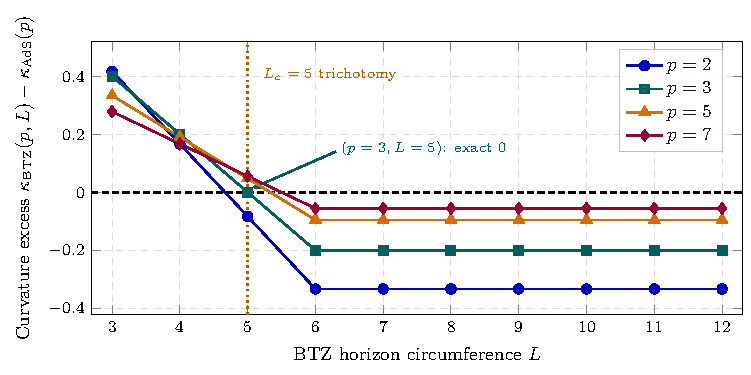
\includegraphics[width=0.92\textwidth]{figures/fig1_btz_curvature.pdf}
  \caption{Exact Tate-curve BTZ horizon curvature excess $\kappa_{\mathrm{BTZ}}(p, L) - \kappa_{\mathrm{AdS}}(p)$ from \cref{thm:btz-ricci} across primes $p \in \{2,3,5,7\}$ and horizon circumferences $L \in [3, 12]$, highlighting Planck-scale flattening ($L \in \{3,4\}$), the exact $L_c = 5$ trichotomy (including exact zero cancellation at $p=3, L=5$), and macroscopic hyperbolicity ($L \ge 6$).}
  \label{fig:btz}
\end{figure}

% =====================================================================
\section[Ryu--Takayanagi Strong Subadditivity and Observatory]{Universal Holographic Ryu--Takayanagi Strong Subadditivity, Gravity, and Observatory}
\label{sec:rt-gravity}
% =====================================================================

In discrete holographic tensor networks~\cite{RyuTakayanagi2006,Heydeman2018,Pastawski2015}, each bulk edge $e = (u, v)$ carries entanglement capacity $c_e = w_e \ln p \ge 0$, and the holographic entanglement entropy of a boundary region $A \subset \partial G$ is the minimum homologous cut capacity $S(A) := \min_{W \sim A} \mathrm{cut}(W)$ where $W \sim A$ means $W|_{\partial G} = A$. Our \code{computeRyuTakayanagi} computes $\gamma_A$ and $\mathcal{E}(A)$ in exact $O(V)$ time via bottom-up tree DP plus a $2$-case BTZ cycle DP (verified against $4{,}096$-state brute-force search in \code{Theorem~8}; Lean~4 certifies exact uniform BTZ engulfing thresholds \code{rt\_uniform\_odd\_prime\_all\_arcs}, \code{rt\_uniform\_dyadic\_two\_arcs}, and complement symmetry $S(A) = S(A^c)$ via \code{rt\_cut\_complement\_symmetry}). We also machine-verify the discrete graph-theoretic form of Headrick and Takayanagi's holographic strong subadditivity theorem~\cite{HeadrickTakayanagi2007}:

\begin{theorem}[Universal Discrete Holographic Ryu--Takayanagi Strong Subadditivity]
\label{thm:rt-ssa}
Let $G = (V, E, c)$ be \emph{any} finite graph with non-negative edge capacities $c_e \ge 0$ and boundary vertex set $\partial G \subseteq V$ (including pure Bruhat--Tits trees, curved AdS metrics, rotating Tate-curve BTZ black holes, and higher-genus Schottky quotients). For any boundary subsets $A, B, C \subseteq \partial G$ with $A \cap C = \emptyset$, and any homologous bulk wedges $W_{AB} \sim A \cup B$ and $W_{BC} \sim B \cup C$,
\begin{equation}
  S(A \cup B \cup C) + S(B) \;\le\; \mathrm{cut}(W_{AB}) + \mathrm{cut}(W_{BC}),
  \label{eq:rt-ssa}
\end{equation}
and hence $S(A \cup B \cup C) + S(B) \le S(A \cup B) + S(B \cup C)$ (setting $B = \emptyset$ gives subadditivity $S(A \cup C) \le S(A) + S(C)$).
\end{theorem}

\begin{proof}
For every single edge $e = (u, v)$ and arbitrary Boolean vertex cuts $X, Y : V \to \{0, 1\}$, exhaustive Boolean case analysis proves pointwise edge submodularity:
\[
  \mathbf{1}_{(X \cup Y)(u) \ne (X \cup Y)(v)} + \mathbf{1}_{(X \cap Y)(u) \ne (X \cap Y)(v)}
  \;\le\;
  \mathbf{1}_{X(u) \ne X(v)} + \mathbf{1}_{Y(u) \ne Y(v)}
\]
(\code{rt\_edge\_cut\_submodular}). Summing over any finite weighted edge list yields global cut submodularity $\mathrm{cut}(W_{AB} \cup W_{BC}) + \mathrm{cut}(W_{AB} \cap W_{BC}) \le \mathrm{cut}(W_{AB}) + \mathrm{cut}(W_{BC})$ (\code{rt\_cut\_submodular}). Because $A \cap C = \emptyset$ on $\partial G$, $(W_{AB} \cup W_{BC})|_{\partial G} = A \cup B \cup C$ (\code{rt\_union\_homologous}) and $(W_{AB} \cap W_{BC})|_{\partial G} = B$ (\code{rt\_inter\_homologous\_disjoint}). By minimality of $S(A \cup B \cup C)$ and $S(B)$, inequality~\eqref{eq:rt-ssa} follows immediately (\code{rt\_strong\_subadditivity}, \code{rt\_subadditivity}, and comparator target \code{target\_thm6\_holographic\_ssa}, zero custom axioms). Independently verified over all $4{,}352$ exhaustive boundary partitions on weighted tree and cyclic BTZ graphs (\code{scripts/verify\_exact.py}) and $1{,}000$ random curved/BTZ JS graphs (\code{test/properties.mjs}).
\end{proof}

Motivated by Gubser--Heydeman--Jepsen--Marcolli edge-length dynamics~\cite{GubserEdge2017}, each edge carries a dynamical log-length $\sigma_e = \ln a_e$ obeying a damped second-order wave equation updated via symmetric Jacobi snapshots (\code{\_sigmaSnap}, Mutant~M7) driven by covariant stress-energy $T_e = w_e|\phi_u - e^{i A_{uv}}\phi_v|^2$, feeding radial redshift backreaction $V_{\mathrm{grav}}(\ell)$ into a fourth-order Yoshida symplectic boundary integrator~\cite{Yoshida1990} (norm drift $\sim 10^{-15}$, verified $\Delta t^4$ energy scaling, Mutant~M5). On curved BTZ horizons, exact bipartite $1$-Wasserstein transport is computed by Johnson potential-reduced Dijkstra ($O(V^2)$ with non-negative reduced costs $r_c = \max(0, c_{uv} + \pi_u - \pi_v)$, eliminating floating-point negative-cycle divergence under extreme $a_e > 24\times$ throat distortions; stress-tested across $200$ extreme curved-BTZ trials). The full coupled system runs live at $60\text{ FPS}$ ($0.654\text{ ms}$ median step on Intel Core Ultra 9 275HX vs.\ $16.67\text{ ms}$ frame budget) in custom zero-dependency WebGL2 GLSL~300~es shaders (\code{src/web/renderer3d.js})---hosted live via GitHub Pages at \url{https://0thernes.github.io/ultrametrica/} alongside an interactive Lean~4 proof dependency blueprint (\url{https://0thernes.github.io/ultrametrica/web/blueprint.html}), WCAG~2.2~AA accessibility, reproducible URL permalinks, PNG capture, a synchronized Euclidean $\R$ twin oscilloscope, and a lock-free $48\text{ kHz}$ \code{AudioWorklet} synthesizer tuned to prime-power Vladimirov harmonic shells ($3^x$ tritaves, $5^x$ pentaves, $7^x$ heptaves) via overflow-immune $O(1)$ log-space folding.

% =====================================================================
\section{Reproducible Benchmarks and Pre-Registered Statistical Falsification}
\label{sec:benchmarks}
% =====================================================================

All reproducible benchmark outputs are archived in \code{results/}: Experiments~A--H via \code{npm run discover} (\code{discovery-\allowbreak benchmarks.json}), latency budgets via \code{npm run bench} (\code{perf-\allowbreak benchmarks.json}), and pre-registered Experiment~I via \code{npm run stats} (\code{stats-\allowbreak eval.json}).

\begin{table}[ht]
\centering
\caption{Experiment~A: Exact Jacobi spectrum of the Monna-conjugated Adelic hybrid Hamiltonian $H_\theta$ ($\alpha = 1.0$), confirming \cref{thm:adelic}.}
\label{tab:adelic}
\footnotesize
\setlength{\tabcolsep}{4.5pt}
\begin{tabular}{@{}rrrrrrr@{}}
\toprule
$p$ & $N$ & $\|[H_Q,H_R]\|_F^{\mathrm{norm}}$ & Distinct ($\theta{=}0$) & Distinct ($\theta{=}0.5$) & Distinct ($\theta{=}1$) & $N\cdot\overline{\IPR}$ ($\theta{=}0.5{\to}1$) \\
\midrule
$2$ & $64$  & $0.02524$ & $33/64$  & $\mathbf{64/64}$ (lifted)   & $7/64$  & $1.424 \to 2.965$ \\
$3$ & $81$  & $0.02187$ & $41/81$  & $\mathbf{41/81}$ (doublets) & $5/81$  & $1.678 \to 3.738$ \\
$5$ & $125$ & $0.01353$ & $63/125$ & $\mathbf{63/125}$ (doublets)& $4/125$ & $1.635 \to 4.967$ \\
\bottomrule
\end{tabular}
\end{table}

\begin{figure}[ht]
  \centering
  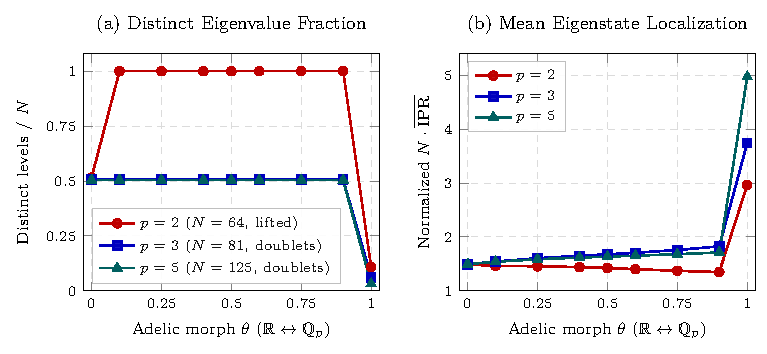
\includegraphics[width=0.98\textwidth]{figures/fig2_adelic_spectrum.pdf}
  \caption{Adelic Parity-Doubling Dichotomy across $\theta \in [0, 1]$: (a)~distinct eigenvalue fraction remains locked at $(N+1)/(2N)$ for odd primes $p=3,5$ while jumping to $1.00$ (complete lifting) at $p=2$; (b)~mean normalized eigenstate localization $N\cdot\overline{\IPR}$.}
  \label{fig:adelic}
\end{figure}

\begin{table}[ht]
\centering
\caption{Experiment~E: Large-$N$ single-sector complex Hermitian Jacobi statistics inside $W_{0,m}$ (cross-validated against full $81\times 81$ real Jacobi to $2.13\times 10^{-14}$), confirming \cref{prop:picket}.}
\label{tab:frontier}
\footnotesize
\setlength{\tabcolsep}{4.5pt}
\begin{tabular}{@{}rrrrrrr@{}}
\toprule
$(p, n, m)$ & $N$ & $\dim W_{0,m}$ & Cross-block leak & $r_0(p,m)$ & $\langle r \rangle(\theta{=}0.5)$ & $\langle r \rangle(\theta{=}0.9)$ \\
\midrule
$(2, 7, 1)$ & $128$ & $64$  & $2.61\times 10^{-15}$ & $0.0000$ & $0.0031$ & $0.0067$ \\
$(2, 8, 1)$ & $256$ & $128$ & $5.04\times 10^{-15}$ & $0.0000$ & $0.0015$ & $0.0193$ \\
$(3, 5, 1)$ & $243$ & $81$  & $5.64\times 10^{-15}$ & $0.5000$ & $0.5039$ & $0.4809$ \\
$(5, 4, 1)$ & $625$ & $125$ & $1.76\times 10^{-14}$ & $0.6667$ & $0.6263$ & $0.6180$ \\
$(5, 4, 2)$ & $625$ & $125$ & $1.43\times 10^{-14}$ & $0.2500$ & $\mathbf{0.2612}$ & $0.2605$ \\
\bottomrule
\end{tabular}
\end{table}

\begin{table}[ht]
\centering
\caption{Pre-registered Experiment~I (sealed in git commit \code{c171b1b} prior to execution; sensitivity additions logged in \code{DEVIATIONS.md}): $20$-seed GUE/GOE controls (\code{seeds 1001..1020}) with $10{,}000$-resample permutation tests, tie-corrected Mann--Whitney~$U$, $95\%$ bootstrap CIs for all three effect sizes ($\Delta\langle r\rangle$, Cliff's $\delta$, Cohen's $d$), Holm--Bonferroni correction~\cite{Holm1979}, and non-pseudoreplicated matrix-level sensitivity tests ($K = 20$ independent control matrices: exact sign/Wilcoxon $p_{\mathrm{exact}} = 1.91\times 10^{-6}$, $p_{\mathrm{Holm}} = 7.63\times 10^{-6}$, empirical rank $p = 1/21$). All $4/4$ hypotheses confirmed ($20/20$ seeds each).}
\label{tab:expi}
\scriptsize
\setlength{\tabcolsep}{2.8pt}
\renewcommand{\arraystretch}{1.15}
\begin{tabular}{@{}lrrrrrrr@{}}
\toprule
Hypothesis & \begin{tabular}[b]{@{}r@{}}$\Delta\langle r\rangle$\\$[95\%\text{ CI}]$\end{tabular} & \begin{tabular}[b]{@{}r@{}}Cliff's $\delta$\\$[95\%\text{ CI}]$\end{tabular} & \begin{tabular}[b]{@{}r@{}}Cohen's $d$\\$[95\%\text{ CI}]$\end{tabular} & MW $p$ & $z_{\mathrm{mat}}$ & $p_{\mathrm{Holm}}$ & Verdict \\
\midrule
H1: $W_{0,2}$ ($5,1.0$) vs.\ GUE & \begin{tabular}[t]{@{}r@{}}$-0.3330$\\$[-0.350,-0.315]$\end{tabular} & \begin{tabular}[t]{@{}r@{}}$-0.8035$\\$[-0.838,-0.763]$\end{tabular} & \begin{tabular}[t]{@{}r@{}}$-1.4786$\\$[-1.566,-1.390]$\end{tabular} & $3.2{\times}10^{-51}$ & $-13.26$ & $0.0004$ & Confirmed \\
\addlinespace[3pt]
H2: $W_{0,1}$ ($5,1.0$) vs.\ GOE & \begin{tabular}[t]{@{}r@{}}$+0.1004$\\$[+0.070,+0.128]$\end{tabular} & \begin{tabular}[t]{@{}r@{}}$+0.2686$\\$[+0.197,+0.336]$\end{tabular} & \begin{tabular}[t]{@{}r@{}}$+0.4059$\\$[+0.280,+0.523]$\end{tabular} & $4.8{\times}10^{-7}$  & $+4.70$  & $0.0004$ & Confirmed \\
\addlinespace[3pt]
H3: $W_{0,1}$ ($2,1.0$) vs.\ GOE & \begin{tabular}[t]{@{}r@{}}$-0.5433$\\$[-0.558,-0.528]$\end{tabular} & \begin{tabular}[t]{@{}r@{}}$-0.9980$\\$[-1.000,-0.993]$\end{tabular} & \begin{tabular}[t]{@{}r@{}}$-2.2329$\\$[-2.325,-2.148]$\end{tabular} & $3.2{\times}10^{-40}$ & $-13.10$ & $0.0004$ & Confirmed \\
\addlinespace[3pt]
H4: $W_{0,2}$ ($5,2.0$) vs.\ GUE & \begin{tabular}[t]{@{}r@{}}$-0.3380$\\$[-0.351,-0.325]$\end{tabular} & \begin{tabular}[t]{@{}r@{}}$-0.8184$\\$[-0.844,-0.792]$\end{tabular} & \begin{tabular}[t]{@{}r@{}}$-1.5037$\\$[-1.574,-1.435]$\end{tabular} & $4.4{\times}10^{-53}$ & $-13.46$ & $0.0004$ & Confirmed \\
\bottomrule
\end{tabular}
\end{table}

\begin{figure}[ht]
  \centering
  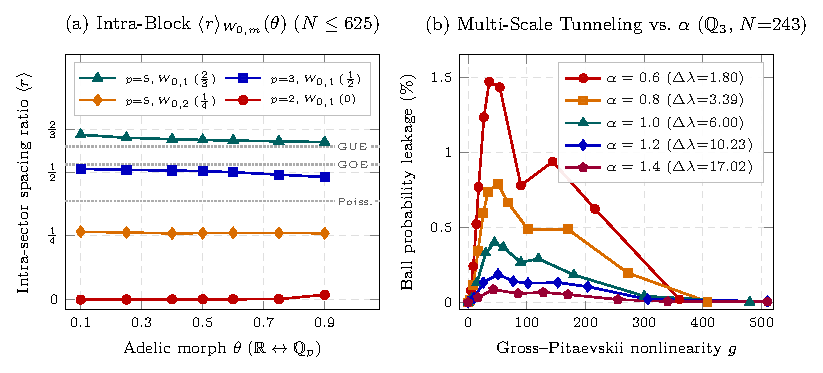
\includegraphics[width=0.98\textwidth]{figures/fig4_intrablock_and_scaling.pdf}
  \caption{Resolution of Open Frontiers \#1 and \#2: (a)~Experiment~E intra-sector spacing ratio $\langle r \rangle_{W_{0,m}}(\theta)$ up to $N = 625$, demonstrating modular picket-fence locking ($W_{0,1} \approx \frac{2}{3}$ vs.\ $W_{0,2} \approx \frac{1}{4}$ inside the same $p=5$ Hamiltonian) rather than GOE/GUE thermalization; (b)~Experiment~F monotonic decay of multi-scale tunneling peaks across $\alpha \in [0.6, 1.4]$ ($\Q_3$, $N=243$) and universal large-$g$ self-trapping.}
  \label{fig:frontier}
\end{figure}

\begin{table}[ht]
\centering
\caption{Experiment~C ($p=3, n=5$): Exact multi-ball Kozyrev compacton-soliton zero leakage vs.\ overlapping multi-scale tunneling resonance and synchronized Euclidean $\R$ twin explosion.}
\label{tab:soliton}
\footnotesize
\setlength{\tabcolsep}{5pt}
\begin{tabular}{@{}rrrrr@{}}
\toprule
$g$ & Solo Soliton ($\Q_3$) & Disjoint 2-Ball Drift & 2-Scale Overlap Leak & Euclidean $\R$ Twin Leak \\
\midrule
$0$   & $0.00\times 10^{0}$ & $2.30\times 10^{-14}$ & $0.00\%$ & $89.21\%$ \\
$20$  & $0.00\times 10^{0}$ & $1.25\times 10^{-14}$ & $0.20\%$ & $87.49\%$ \\
$60$  & $0.00\times 10^{0}$ & $7.44\times 10^{-15}$ & $\mathbf{0.37\%}$ (peak) & $83.58\%$ \\
$150$ & $0.00\times 10^{0}$ & $2.42\times 10^{-14}$ & $0.29\%$ & $71.45\%$ \\
$300$ & $0.00\times 10^{0}$ & $1.87\times 10^{-14}$ & $0.04\%$ & $61.13\%$ \\
$500$ & $0.00\times 10^{0}$ & $2.35\times 10^{-14}$ & $\mathbf{0.00\%}$ (self-trapped) & $59.40\%$ \\
\bottomrule
\end{tabular}
\end{table}

\begin{figure}[ht]
  \centering
  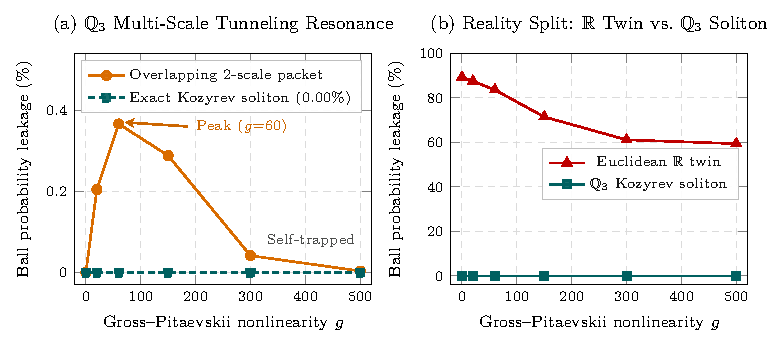
\includegraphics[width=0.98\textwidth]{figures/fig3_soliton_resonance.pdf}
  \caption{Experiment~C ($p=3, n=5$): (a)~non-monotonic multi-scale ultrametric tunneling resonance peaking at $g = 60$ and collapsing via macroscopic self-trapping at $g = 500$, contrasted with exact zero leakage of a single Kozyrev compacton-soliton; (b)~Reality Split comparison against the synchronized Euclidean $\R$ twin.}
  \label{fig:soliton}
\end{figure}

In Experiment~B, exact Johnson potential-reduced Dijkstra bipartite Wasserstein measurements match \cref{thm:btz-ricci} to $\le 2.22\times 10^{-16}$ across all tested horizons $L \in \{3,4,5,7,8,9,16\}$. In Experiment~D ($p=3, n=5, L=9$), sweeping Kerr flux $\Omega \in [-\pi,\pi]$ yields peak horizon current $|J| = 1.1169\times 10^{-2}$ with exact odd current parity $\max|J(-\Omega)+J(\Omega)| = 0.00$ and exact even bulk action $\max|E(-\Omega)-E(\Omega)| = 0.00$.

\begin{figure}[ht]
  \centering
  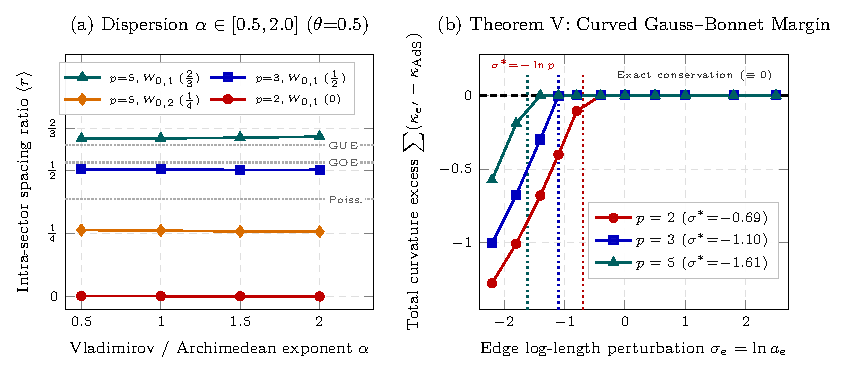
\includegraphics[width=0.98\textwidth]{figures/fig5_spectrum_and_gaussbonnet.pdf}
  \caption{Experiments~G and~H: (a)~$\alpha$-invariance of intra-sector modular picket-fence locking across $\alpha \in \{0.5, 1.0, 1.5, 2.0\}$ at $\theta = 0.5$ up to $N = 625$ (including quadratic Schr\"odinger dispersion $\alpha = 2.0$, where $W_{0,1}$ and $W_{0,2}$ remain locked near $\frac{2}{3}$ and $\frac{1}{4}$); (b)~non-perturbative verification of \cref{thm:gauss-bonnet}, showing exact zero integrated curvature excess for all $\sigma_e \ge -\ln p$ and the exact supercritical negative pinch deficit past $\sigma_e^* = -\ln p$ (error $\le 5.33\times 10^{-15}$).}
  \label{fig:gaussbonnet}
\end{figure}

In Experiment~H, curved bridge Ollivier--Ricci curvature-excess sums match \cref{thm:gauss-bonnet} to $7.77\times 10^{-16}$ ($p=2$), $1.33\times 10^{-15}$ ($p=3$), and $5.33\times 10^{-15}$ ($p=5$), while sweeping the conformal dimension down to $\Delta = 0.5001$ ($m^2 - m_{\mathrm{BF}}^2 \approx 2.09\times 10^{-8}$) under inhomogeneous curved gravity ($\sigma_e \in [-1.5, 1.5]$) and maximal Kerr flux ($\Omega = \pi$) maintains worst uneliminated Klein--Gordon residual $5.38\times 10^{-15}$ and minimum Schur pivot $0.8637 > 0$.

\FloatBarrier

% =====================================================================
\section[Formal Audit, Limitations, and Provenance]{Multi-Kernel Lean~4 Audit, Limitations, Reproducibility, and Governance}
\label{sec:audit}
% =====================================================================

\begin{table}[ht]
\centering
\caption{Lean~4 (\code{v4.35.0}, Palomar \code{module}, \code{autoImplicit = false}, all $17$ files $< 1{,}000$ lines) formalization map: $250$ audited declarations ($100.0\%$ public theorem coverage; $0$ unaudited) transparently classified into $144$ core theorems/corollaries, $81$ zero-Mathlib helper lemmas, $10$ adversarial refutations, and $15$ isolated \code{Challenge}/\code{Solution} comparator bindings (re-verifications from pure \code{Spec.lean}, never double-counted as separate theorems; zero Mathlib, zero \code{native\_decide}, zero \code{sorryAx}, zero custom axioms).}
\label{tab:lean}
\scriptsize
\renewcommand{\arraystretch}{0.94}
\setlength{\tabcolsep}{3.0pt}
\begin{tabular}{@{}>{\raggedright\arraybackslash}p{3.4cm}>{\raggedright\arraybackslash}p{6.8cm}r>{\raggedright\arraybackslash}p{3.3cm}@{}}
\toprule
Module & Key Audited Declarations & Count & Axioms Used \\
\midrule
\code{Basic.lean} & \code{monna\_involution\_universal}, \code{monna\_injective}, \code{padic\_ball\_monna\_contiguity}, \code{bruhatTits\_leaves\_isosceles} & $26$ & \code{propext}, \code{Classical.choice}, \code{Quot.sound} (or none) \\
\code{AdelicSymmetry.lean} & \code{hilbert\_sector\_completeness}, \code{subtreeShift\_preserves\_ultrametric\_prefix}, \code{picket\_fence\_monotone}, \code{odd\_prime\_conjugate\_sector\_disjoint} & $23$ & \code{propext}, \code{Classical.choice}, \code{Quot.sound} (or none) \\
\code{OperatorAnd\allowbreak Spectrum.lean} & \code{commuting\_diag\_block\_diagonal}, \code{fourierConj\_maps\_sector}, \code{odd\_prime\_sector\_eigenvector\_orthogonal\_doublet}, \code{odd\_prime\_doublet\_linearly\_independent} & $21$ & \code{propext}, \code{Classical.choice}, \code{Quot.sound} (or none) \\
\code{Holography\allowbreak Curvature.lean} & \code{btz\_graph\_metric\_eq\_classDist}, \code{btz\_wasserstein\_lower\_bound}, \code{btz\_primal\_cost\_exact}, \code{gubser\_bf\_bound\_exact\_square}, \code{curved\_ads\_gauss\_bonnet\_subcritical} & $40$ & \code{propext}, \code{Quot.sound} (or none) \\
\code{FullGraphBTZ.lean} & \code{fullBtz\_agg\_feasible}, \code{fullBtz\_cost\_eq\_agg}, \code{fullBtz\_wasserstein\_lower\_bound}, \code{fullBtz\_primal\_optimal\_exists} & $6$ & \code{propext}, \code{Classical.choice}, \code{Quot.sound} \\
\code{MultiEdge\allowbreak Holography.lean} & \code{gen\_bridge\_wasserstein\_lower\_bound\_sub/sup}, \code{gen\_bridge\_primal\_sub/sup\_optimal}, \code{global\_multi\_edge\_vertex\_charge\_conservation}, \code{rt\_strong\_subadditivity} & $33$ & \code{propext}, \code{Classical.choice}, \code{Quot.sound} (or none) \\
\code{FiniteGraph\allowbreak GaussBonnet.lean} & \code{finite\_graph\_half\_charge\_double\_count}, \code{finite\_graph\_curved\_gauss\_bonnet\_sum}, \code{finite\_graph\_subcritical\_gauss\_bonnet\_conserved} & $24$ & \code{propext}, \code{Classical.choice}, \code{Quot.sound} (or none) \\
\code{SolitonAnd\allowbreak Solver.lean} & \code{multi\_ball\_kozyrev\_soliton\_list}, \code{horizon\_edge\_quadratic\_expansion}, \code{sherman\_morrison\_exact\_identity}, \code{kerr\_flux\_edge\_*} (+6 \code{CInt} lemmas) & $18$ & \code{propext}, \code{Quot.sound} (or none) \\
\code{BulkOperator\allowbreak Positivity.lean} & \code{gaugeLaplacianQuad\_nonneg}, \code{bulk\_operator\_strictly\_pos\_def}, \code{spd\_operator\_sherman\_morrison\_den\_ge\_one}, \code{tree\_schur\_pivot\_stays\_positive} & $8$ & \code{propext}, \code{Classical.choice}, \code{Quot.sound} \\
\code{Vladimirov\allowbreak Operator.lean} & \code{padicDistVal\_\allowbreak strong\_\allowbreak tri}, \code{kozyrevHaar\_\allowbreak zero\_\allowbreak mean}, \code{kozyrevHaar\_\allowbreak vladimirov\_\allowbreak eigenfunction}, \code{ultrametricOp\_\allowbreak commutes\_\allowbreak vecRev}, \code{j\_\allowbreak commuting\_\allowbreak preserves\_\allowbreak parity} & $26$ & \code{propext}, \code{Classical.choice}, \code{Quot.sound} (or none) \\
\code{Adversarial\allowbreak Tests.lean} & $10$ kernel-checked false-variant negations across Theorems~I--VII (incl.\ negative full-graph BTZ, dyadic non-orthogonality, negative-mass $T$) & $10$ & \code{propext}, \code{Quot.sound} (or none) \\
\code{Spec}, \code{Challenge}, \code{Solution} & $15$ isolated bindings (Targets~1--12 + full-graph BTZ~T13, operator doublets~T14, bulk $T\succ 0$/Schur~T15, $13/13$ non-vacuity) & $15$ & Verified across $6$ independent kernels \\
\bottomrule
\end{tabular}
\end{table}

\textbf{Multi-Kernel Statement Fidelity, Negative Tamper Rejection, and Verification Boundaries.} To eliminate single-kernel trust risks on the headline targets, every Lean file uses Palomar Registry \code{module} headers and stays strictly under $1{,}000$ lines ($17$ files, max $955$ lines); \code{Spec.\allowbreak lean} isolates pure definitions (zero proofs), \code{Challenge.\allowbreak lean} states all $15$ targets importing only \code{Spec}, and sorry-free \code{Solution.\allowbreak lean} (bridged via modular \code{Solution\allowbreak Bridge.\allowbreak lean}) proves them identically---including tight $3$-class and literal $(p+2)\times(p+2)$ full-graph BTZ primal attainment (Targets~3, 13), operator-level block-diagonality and odd-prime orthogonal doublet multiplicity $\ge 2$ over $\Z[i]^N$ (Target~14), bulk gauge-covariant Laplacian strict positive definiteness $T \succ 0$, end-to-end Sherman--Morrison $\mathrm{den} \ge 1$ discharge, and \code{RatQ} tree Schur-complement pivot positivity (Target~15), abstract arbitrary-dimension $L$ complex Hermitian Sherman--Morrison, non-negative subcritical and supercritical bridge-edge primal attainment, direct finite-graph edge-sum bridge Ollivier--Ricci subcritical metric-invariance (Target~11), first-principles discrete Vladimirov and Kozyrev--Haar eigenfunctions and $[D_K, J] = 0$ parity preservation (Target~12), and concrete non-vacuity witnesses covering all $13$ theorem targets. Every single public theorem across all $11$ proof modules and \code{Solution.\allowbreak lean} ($250/250$, $100.0\%$ coverage, enforced automatically by \code{verify\_\allowbreak exact.\allowbreak py}) passes Lean~4~\cite{deMouraUllrich2021} (\code{v4.35.0}) and \code{leanchecker {-}{-}fresh} locally under strict \code{[propext, Quot.\allowbreak sound, Classical.\allowbreak choice]}, while GitHub Actions CI enforces \code{lake check {-}{-}paranoid} on the full package, $6$-kernel \code{lake comparator {-}{-}paranoid} (\code{lean4}, \code{leanchecker}, \code{lean4lean}, \code{con-leche}, \code{con-ron}, \code{nanoda\_\allowbreak bin}) across all $15$ comparator targets and their dependency closure inside a Linux \code{bubblewrap} sandbox, and a live negative tamper-rejection gate (\code{scripts/\allowbreak test\_\allowbreak lean\_\allowbreak negative.\allowbreak py}) confirming that injected \code{sorry} proofs and weakened \code{Challenge.\allowbreak lean} signatures are actively rejected (\code{docs/\allowbreak statement-\allowbreak fidelity.\allowbreak md}; live dependency DAG at \href{https://0thernes.github.io/ultrametrica/web/blueprint.html}{0thernes.\allowbreak github.\allowbreak io/\allowbreak ultrametrica/\allowbreak web/\allowbreak blueprint.\allowbreak html}, verified by \code{scripts/\allowbreak check\_\allowbreak blueprint.\allowbreak py}). Lean formalizes invariants of the repository's own discrete algebraic models (crediting Monna~\cite{Monna1970}, Kozyrev~\cite{Kozyrev2002}, and Headrick--Takayanagi~\cite{HeadrickTakayanagi2007}); operating strictly over exact rings ($\Z, \Z[i], \text{\code{RatQ}}$), it still does not formalize the full irrational-root DFT matrix $H_\theta$, continuum PDE time evolution, the floating-point $O(V)$ JS solver implementation, or tachyonic negative-mass BF-window positivity ($m^2 \in (m_{\mathrm{BF}}^2, 0)$). A nested-comment- and string-aware scanner in \code{verify\_\allowbreak exact.\allowbreak py} confirms zero forbidden tokens (\code{sorry}, \code{admit}, \code{axiom}, \code{native\_\allowbreak decide}, \code{unsafe}, \code{implemented\_\allowbreak by}, \code{@[extern}) across all sorry-free Lean files, zero unaudited public Lean theorems, and zero broken internal Markdown links; \code{check\_\allowbreak readme\_\allowbreak axioms.\allowbreak py} checks the verbatim \code{\#print axioms} lines in \code{README.\allowbreak md} against \code{lean4-\allowbreak audit.\allowbreak txt}, and \code{check\_\allowbreak citations.\allowbreak py {-}{-}live} audits all $21/21$ BibTeX--LaTeX entries plus live Crossref title/author/retraction metadata and arXiv \code{eprint} title/author resolution ($18/18$ DOIs HTTP~200, min title Jaccard $1.00$, $0$ retractions, $11/11$ arXiv \code{eprint} IDs verified, archived in \code{results/\allowbreak citation-\allowbreak audit.\allowbreak json}). Outside the Lean kernel, \code{verify\_\allowbreak exact.\allowbreak py} checks exact \code{Fraction}, $\Q(i)$, exact integer discrete Vladimirov/Kozyrev--Haar, and brute-force invariants ($7{,}033$ pairs, $45$ BTZ horizons, $69$ curved trees, $4{,}352$ RT SSA partitions), \code{padic\_\allowbreak oracle.\allowbreak py} cross-checks $1{,}000+$ differential queries, \code{tsc {-}{-}noEmit} confirms zero strict-mode JSDoc type errors across \code{src/\allowbreak engine/\allowbreak *.js}, and \code{test/\allowbreak *.mjs} runs $36$ Node suites ($10$ theorems, $12/12$ real source-code mutants killed against unmodified \code{test/\allowbreak verify.\allowbreak mjs}, $3{,}400+$ property, metamorphic, curved-BTZ stress, and negative checks, $1{,}000$ deterministic HTTP/engine fuzz cases, $3$ parallel HTTP/\code{AudioWorklet} concurrency suites, HTTP contract plus disk \code{EIO} failure injection and \code{favicon.\allowbreak svg}, and golden snapshots).

\textbf{Limitations, Relation to Open Problems, and Threats to Validity.} Full limitations, a literal-vs.-metaphor separation table, and a 43-item independent research readiness audit are documented in \code{LIMITATIONS.md} and \code{SUBMISSION\_READINESS.md}. Specifically: (1)~no full solution to any open problem in \code{unsolved-problems-mega-atlas} is claimed ($0/1{,}900$; \code{docs/\allowbreak MEGA\_ATLAS\_CROSSCHECK.\allowbreak md}); (2)~asymptotic $n \to \infty$ analytic convergence of $\langle r\rangle_{W_{0,m}} \to r_0(p,m)$ for $\alpha \ne 1$ is verified numerically (\code{numerical\_approximation}) and statistically up to $N = 625$ rather than proved in Lean; (3)~adjacent level-spacing ratios within one matrix exhibit weak lag-1 correlation, which we explicitly address via our non-pseudoreplicated $20$-matrix sensitivity analysis in \code{DEVIATIONS.md} and \cref{tab:expi}; (4)~\cref{thm:gauss-bonnet-global} is local vertex-normalization telescoping on strictly interior bridges of full degree $p+1$ (excluding finite-cutoff leaf edges, which are unconditionally supercritical; see \cref{rem:gubser-non-topological}); and (5)~real-time WebGL2 visualization is capped at $N \le 343$ due to $O(N^2)$ visual panels, while \code{PadicSpace} enforces $N \le 65{,}536$.

\newpage
\textbf{Reproducibility, Cryptographic Timestamps, Authorship (CRediT), Funding, COI, Export-Control, and AI Disclosure.} Every theorem, figure, benchmark, statistical test, PDF, and bit-identical deterministic arXiv tarball (\code{scripts/package\_dist.py}) is reproduced from a clean clone via \code{just reproduce} (logged in \code{REPLICATION.md}, pinned in \code{CHECKSUMS.\allowbreak sha256} and \code{data/\allowbreak MANIFEST.\allowbreak sha256}, and externally sealed by dual independent cryptographic timestamps via DigiCert RFC~3161 \code{data/CHECKSUMS.sha256.tsr} and 3-calendar Bitcoin OpenTimestamps \code{data/CHECKSUMS.sha256.ots}, offline-verified by \code{scripts/stamp\_manifest.py {-}{-}verify}). \emph{CRediT roles:} Alexander Stephen Donahue (ORCID \code{0009-\allowbreak 0006-\allowbreak 8168-\allowbreak 9648})---Conceptualization, Supervision, Validation, Project Administration, Software \& Formal Verification Direction, and Writing -- Review \& Editing. \emph{AI-Assistance \& Provenance Disclosure:} Substantive AI assistance (Google DeepMind / Antigravity agent under the author's direction) contributed to mathematical derivation, software implementation, Lean~4 formalization, test engineering, and manuscript drafting; AI systems are disclosed as tools and are not listed as authors. Chronological session audit summaries appear in \code{docs/\allowbreak run-log.\allowbreak md} and \code{docs/\allowbreak reviews/}; raw unredacted local transcripts are retained privately on the author's workstation. \emph{Export-Control Self-Screen:} Pure fundamental mathematical physics and educational visualization intended for public release (15~CFR~\S~734.8); zero cryptography, weapons, or dual-use software. \emph{Funding \& COI:} Self-funded independent research (Independent Researcher, Spokane, WA, USA; handle \code{0thernes}; no LLC, corporate, or institutional affiliation asserted); no competing financial interests declared. \emph{Code \& Data Availability:} Publicly archived at \url{https://github.com/0thernes/ultrametrica} and \url{https://github.com/0thernes/0thernes-research-archive} (entry \code{0TH-BUILD-003}) under the Cosmogonic Non-Commercial Research \& Play License (see \code{LICENSE}, \code{LEGAL.md}, \code{DEVIATIONS.md}, and \code{ERRATA.md}).

\clearpage
\bibliographystyle{plain}
\bibliography{refs}

\end{document}
